\begin{EnvFullwidth}
\textit{In Questions~\ref{calc07:area-first}--\ref{calc07:area-last}, choose the alternative that gives the area of the region described.}
\end{EnvFullwidth}

\question\label{calc07:area-first}
The curve of $y=x^{2}, y=0, x=-1$, and $x=2$.
\begin{choices}
  \choice $\dfrac{11}{3}$
  \choice $\dfrac{7}{3}$
  \CorrectChoice $3$
  \choice $5$
  \choice none of these
\end{choices}
\begin{solution}
\begin{center}
  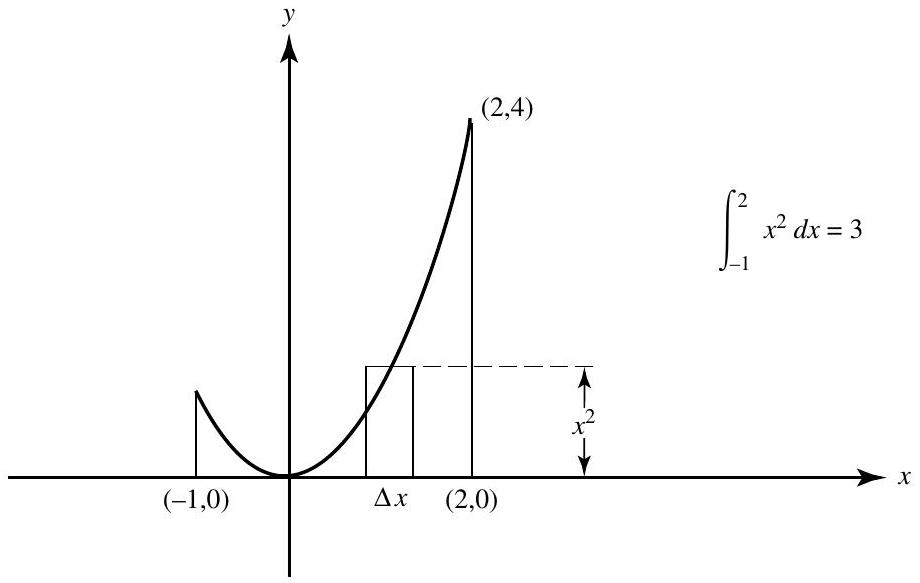
\includegraphics[width=0.50\linewidth]{calculus/images/4dd14383-56bc-4a03-ad67-ca78eb85270b-11_583_920_1345_533.jpg}
\end{center}
\end{solution}


\newpage


\question
The parabola $y=x^{2}-3$ and the line $y=1$.
\begin{choices}
  \choice $\dfrac{8}{3}$
  \choice $32$
  \CorrectChoice $\dfrac{32}{3}$
  \choice $\dfrac{16}{3}$
  \choice none of these
\end{choices}
\begin{solution}
  \begin{center}
    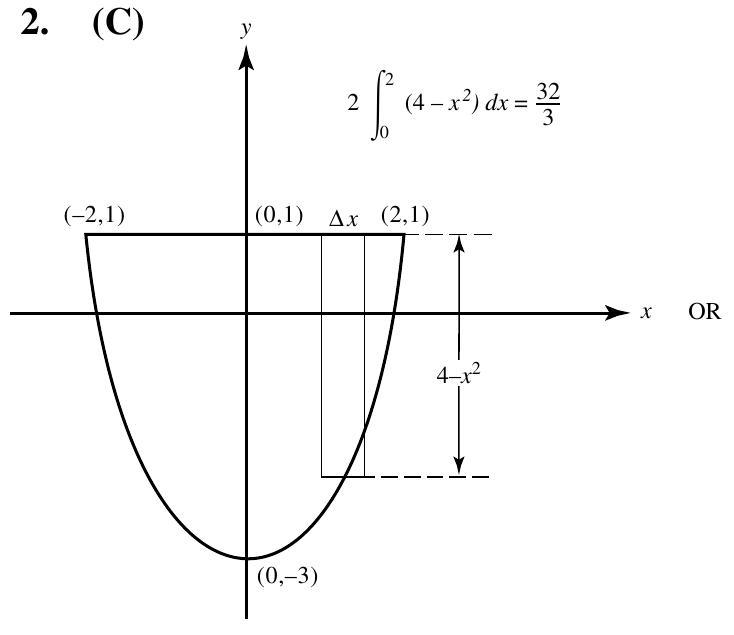
\includegraphics[width=0.50\linewidth]{calculus/images/4dd14383-56bc-4a03-ad67-ca78eb85270b-12_635_734_296_672.jpg}
    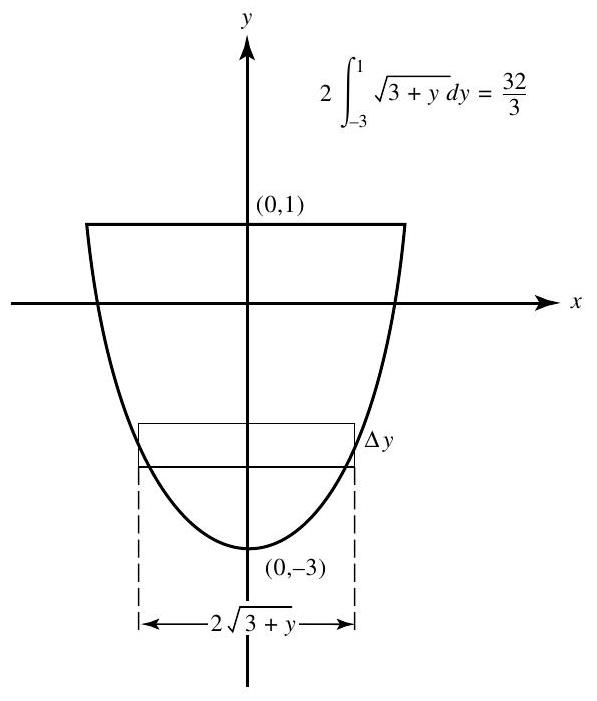
\includegraphics[width=0.50\linewidth]{calculus/images/4dd14383-56bc-4a03-ad67-ca78eb85270b-12_701_597_306_1447.jpg}
  \end{center}
\end{solution}



\newpage




\question
The curve of $x=y^{2}-1$ and the $y$-axis.
\begin{choices}
  \CorrectChoice $\dfrac{4}{3}$
  \choice $\dfrac{2}{3}$
  \choice $\dfrac{8}{3}$
  \choice $\dfrac{1}{2}$
  \choice none of these
\end{choices}
\begin{solution}
  \begin{center}
    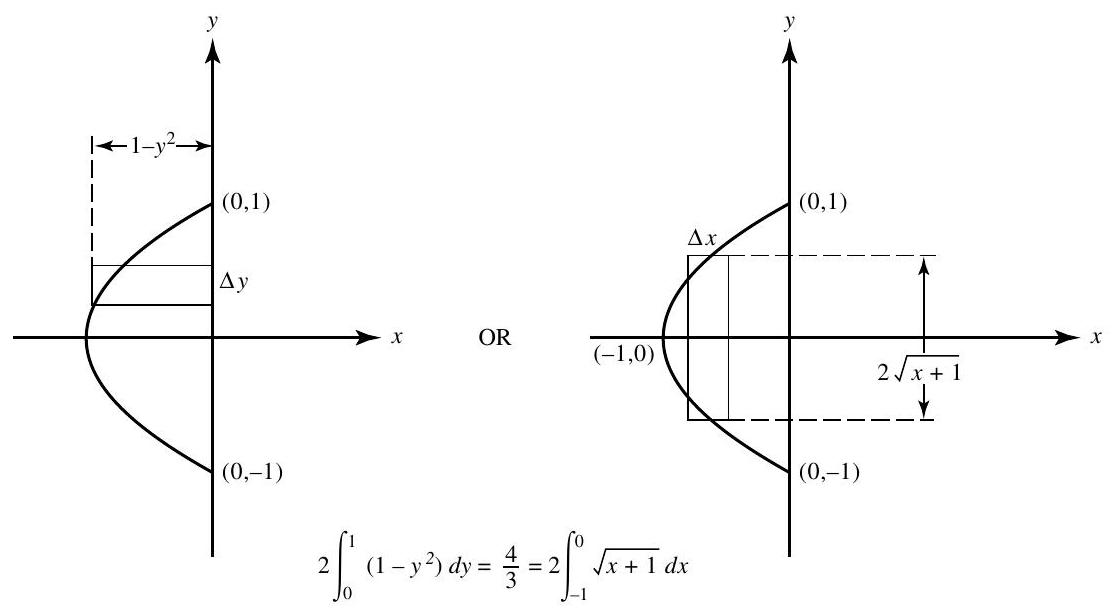
\includegraphics[width=0.70\linewidth]{calculus/images/4dd14383-56bc-4a03-ad67-ca78eb85270b-12_613_1119_1090_835.jpg}
  \end{center}
\end{solution}



\newpage



\question
The parabola $y^{2}=x$ and the line $x+y=2$.
\begin{choices}
  \choice $\dfrac{5}{2}$
  \choice $\dfrac{3}{2}$
  \choice $\dfrac{11}{6}$
  \CorrectChoice $\dfrac{9}{2}$
  \choice $\dfrac{29}{6}$
\end{choices}
\begin{solution}
  \begin{center}
    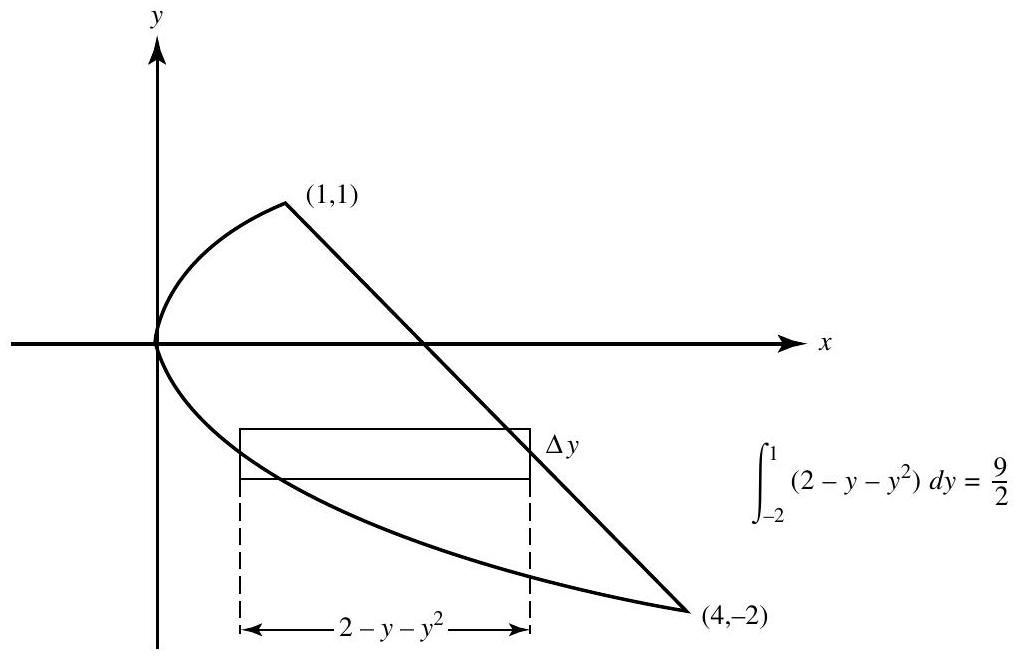
\includegraphics[width=0.70\linewidth]{calculus/images/4dd14383-56bc-4a03-ad67-ca78eb85270b-12_662_1024_1837_874.jpg}
  \end{center}
\end{solution}



\newpage



\question
The curve of $y=\dfrac{4}{x^{2}+4}$, the $x$-axis, and the vertical lines $x=-2$ and $x=2$.
\begin{choices}
  \choice $\dfrac{\pi}{4}$
  \choice $\dfrac{\pi}{2}$
  \choice $2 \pi$
  \CorrectChoice $\pi$
  \choice none of these
\end{choices}
\begin{solution}
  \begin{center}
    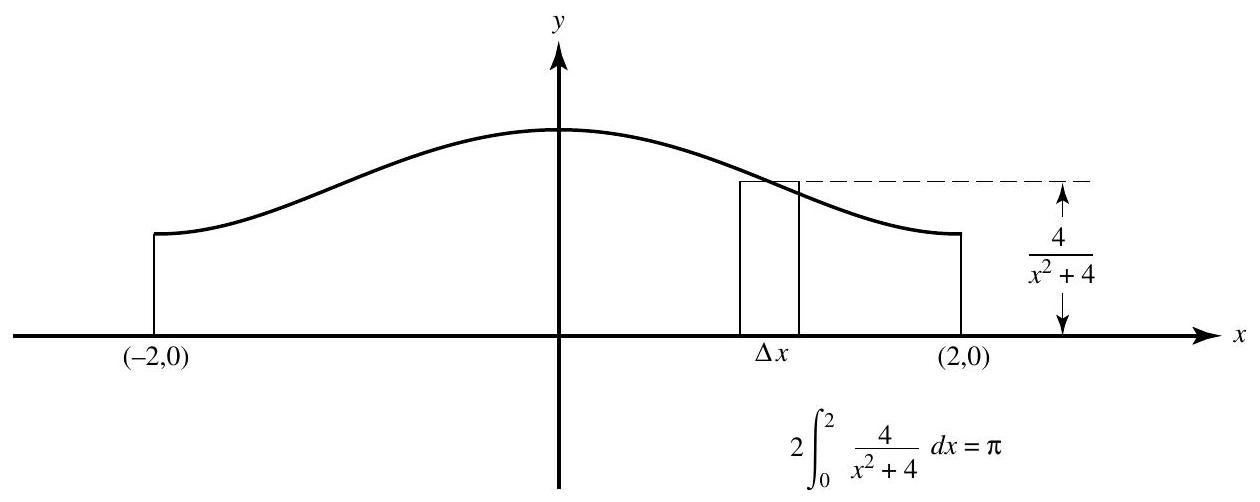
\includegraphics[width=0.70\linewidth]{calculus/images/4dd14383-56bc-4a03-ad67-ca78eb85270b-13_502_1260_308_473.jpg}
  \end{center} 
\end{solution}


\question
The parabolas $x=y^{2}-5 y$ and $x=3 y-y^{2}$.
\begin{choices}
  \choice $\dfrac{32}{3}$
  \choice $\dfrac{139}{6}$
  \CorrectChoice $\dfrac{64}{3}$
  \choice $\dfrac{128}{3}$
  \choice none of these
\end{choices}
\begin{solution}
  \begin{center}
    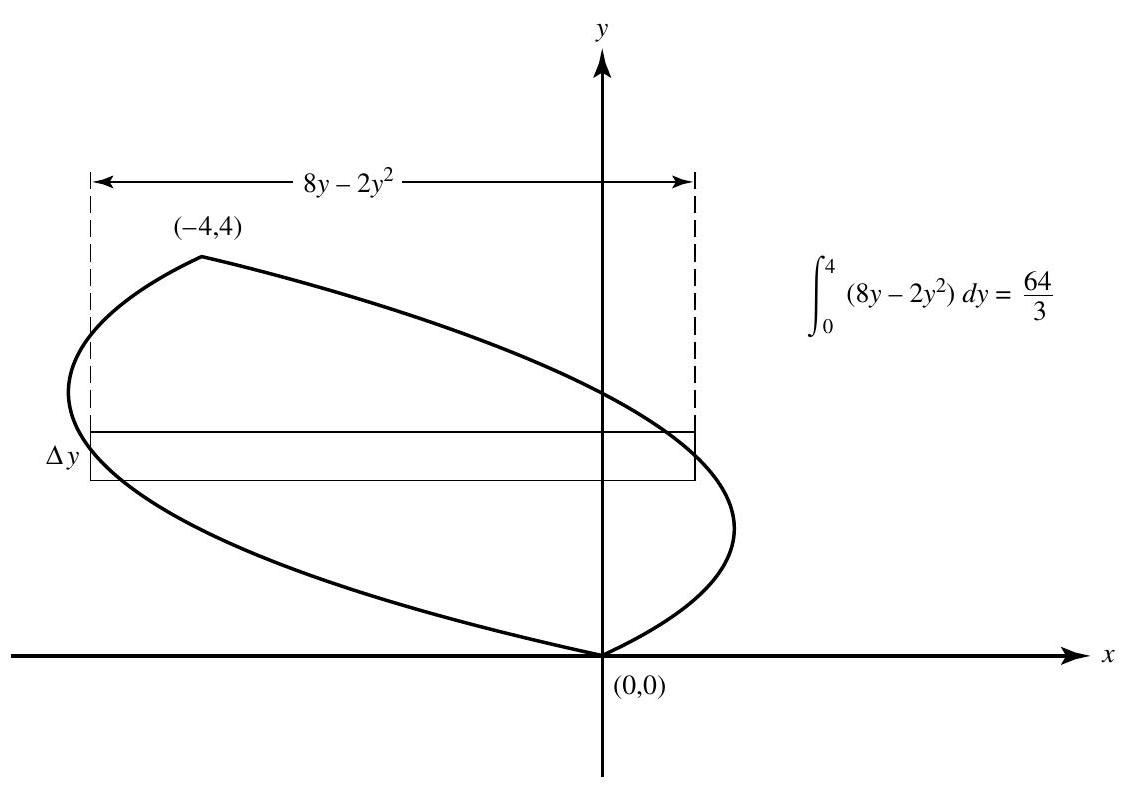
\includegraphics[width=0.50\linewidth]{calculus/images/4dd14383-56bc-4a03-ad67-ca78eb85270b-13_785_1140_920_577.jpg}
  \end{center}
\end{solution}


\newpage

\question
The curve of $y=\dfrac{2}{x}$ and $x+y=3$.
\begin{choices}
  \choice $\dfrac{1}{2}-2 \ln 2$
  \choice $\dfrac{3}{2}$
  \choice $\dfrac{1}{2}-\ln 4$
  \choice $\dfrac{5}{2}$
  \CorrectChoice $\dfrac{3}{2}-\ln 4$
\end{choices}
\begin{solution}
  \begin{center}
    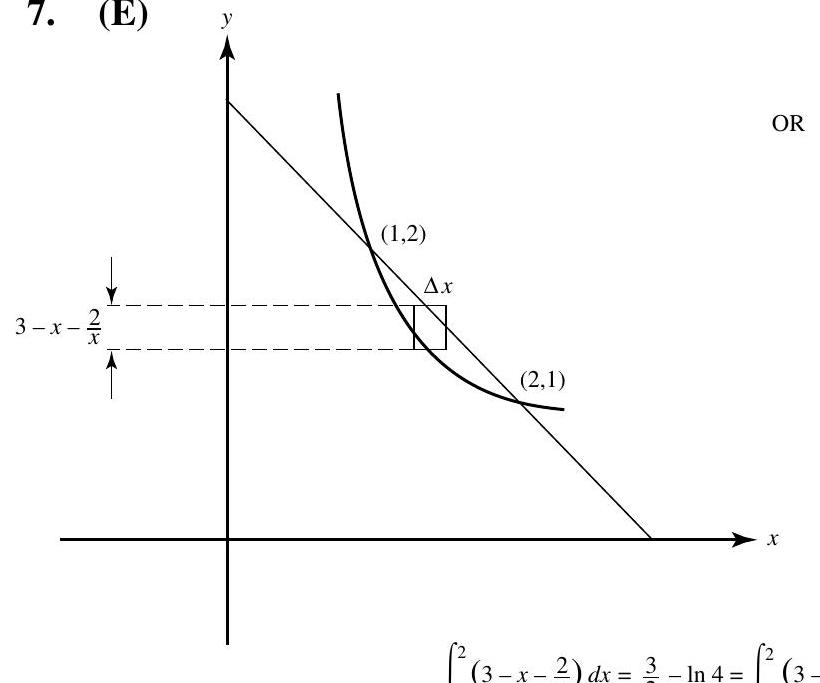
\includegraphics[width=0.50\linewidth]{calculus/images/4dd14383-56bc-4a03-ad67-ca78eb85270b-13_683_820_1774_289.jpg}
  \end{center}
  \begin{center}
    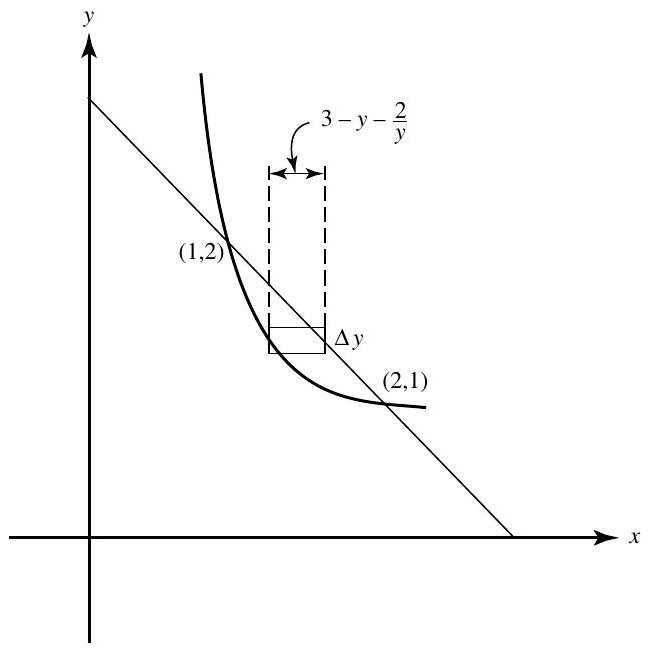
\includegraphics[width=0.50\linewidth]{calculus/images/4dd14383-56bc-4a03-ad67-ca78eb85270b-13_648_657_1776_1127.jpg}
  \end{center}
\end{solution}



\newpage


\question
In the first quadrant, bounded below by the $x$-axis and above by the curves of $y=\sin x$ and $y=\cos x$.
\begin{choices}
  \CorrectChoice $2-\sqrt{2}$
  \choice $2+\sqrt{2}$
  \choice 2
  \choice $\sqrt{2}$
  \choice $2 \sqrt{2}$
\end{choices}

\question
Bounded above by the curve $y=\sin x$ and below by $y=\cos x$ from $x=\dfrac{\pi}{4}$ to $x=\dfrac{5 \pi}{4}$.
\begin{choices}
  \CorrectChoice $2 \sqrt{2}$
  \choice $\dfrac{2}{\sqrt{2}}$
  \choice $\dfrac{1}{2 \sqrt{2}}$
  \choice $2(\sqrt{2}-1)$
  \choice $2(\sqrt{2}+1)$
\end{choices}

\question
The curve $y=\cot x$, the line $x=\dfrac{\pi}{4}$, and the $x$-axis.
\begin{choices}
  \choice $\ln 2$
  \choice $\dfrac{1}{2} \ln \dfrac{1}{2}$
  \choice 1
  \CorrectChoice $\dfrac{1}{2} \ln 2$
  \choice 2
\end{choices}
\begin{solution}
(D)\\
\begin{center}
  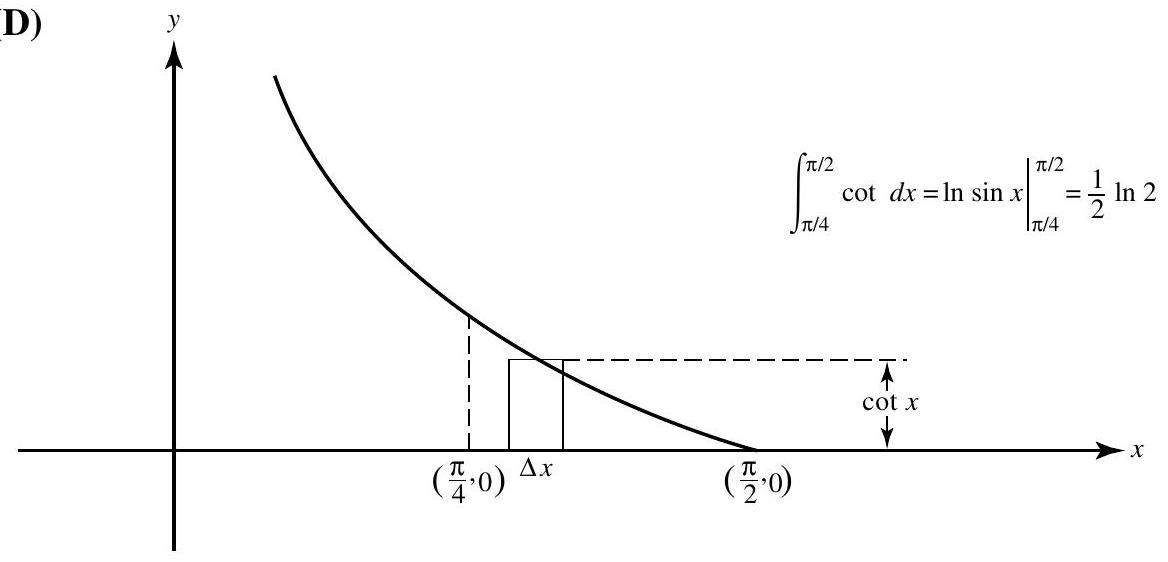
\includegraphics[width=0.50\linewidth]{calculus/images/4dd14383-56bc-4a03-ad67-ca78eb85270b-14_562_1168_1876_649.jpg}
\end{center}
\end{solution}



\newpage



\question\label{calc07:area-last}
The curve of $y=x^{3}-2 x^{2}-3 x$ and the $x$-axis.
\begin{choices}
  \choice $\dfrac{28}{3}$
  \choice $\dfrac{79}{6}$
  \choice $\dfrac{45}{4}$
  \CorrectChoice $\dfrac{71}{6}$
  \choice none of these
\end{choices}
\begin{solution}
(D)\\
\begin{center}
  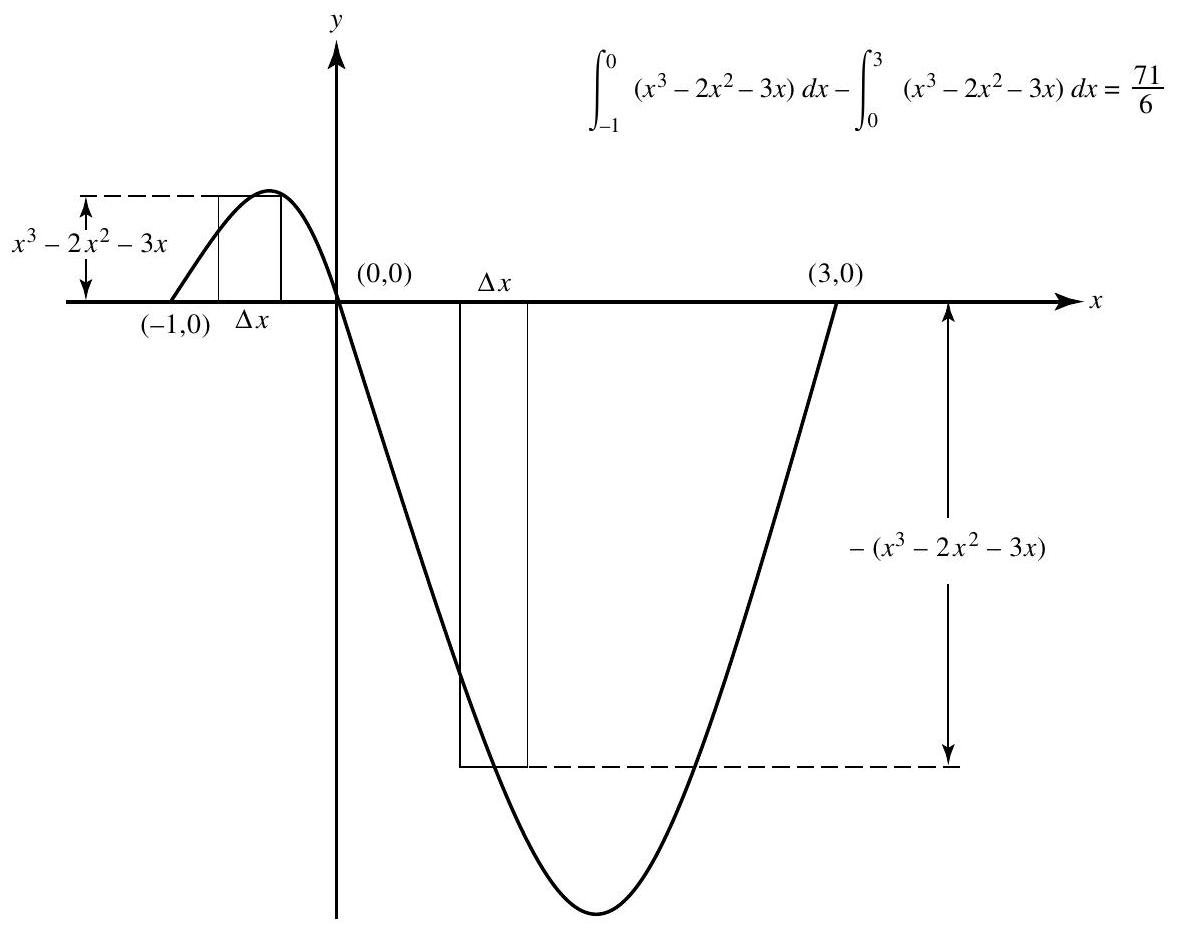
\includegraphics[width=0.50\linewidth]{calculus/images/4dd14383-56bc-4a03-ad67-ca78eb85270b-15_931_1177_301_503.jpg}
\end{center}
\end{solution}

\question
The total area bounded by the cubic $x=y^{3}-y$ and the line $x=3 y$ is equal to
\begin{choices}
  \choice 4
  \choice $\dfrac{16}{3}$
  \CorrectChoice 8
  \choice $\dfrac{32}{3}$
  \choice 16
\end{choices}
\begin{solution}
(C)\\
\begin{center}
  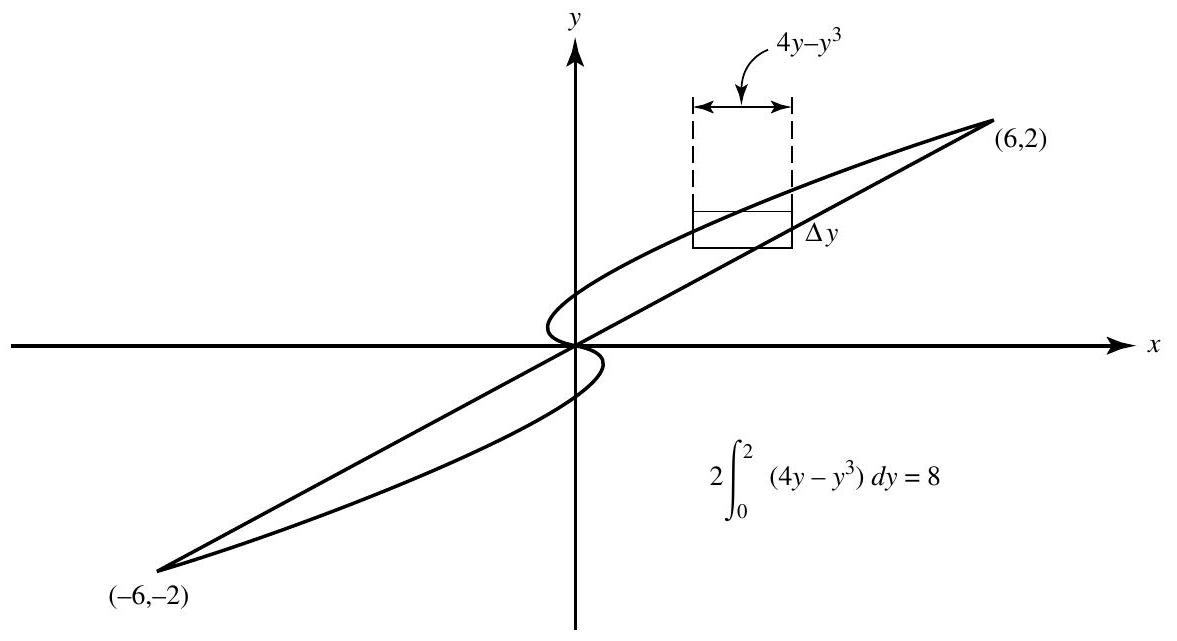
\includegraphics[width=0.50\linewidth]{calculus/images/4dd14383-56bc-4a03-ad67-ca78eb85270b-15_641_1177_1280_484.jpg}
\end{center}
\end{solution}



\newpage




\question
The area bounded by $y=e^{x}, y=2$, and the $y$-axis is equal to
\begin{choices}
  \choice $3-e$
  \choice $e^{2}-1$
  \choice $e^{2}+1$
  \CorrectChoice $2 \ln 2-1$
  \choice $2 \ln 2-3$
\end{choices}
\begin{solution}
(D)
\[
\begin{aligned}
\int_{0}^{\ln 2}\left(2-e^{x}\right) d x & =\left.\left(2 x-e^{x}\right)\right|_{0} ^{\ln 2} \\
& =\left(2 \ln 2-e^{\ln 2}\right)-\left(2 \cdot 0-e^{0}\right) \\
& =2 \ln 2-1
\end{aligned}
\]
\begin{center}
  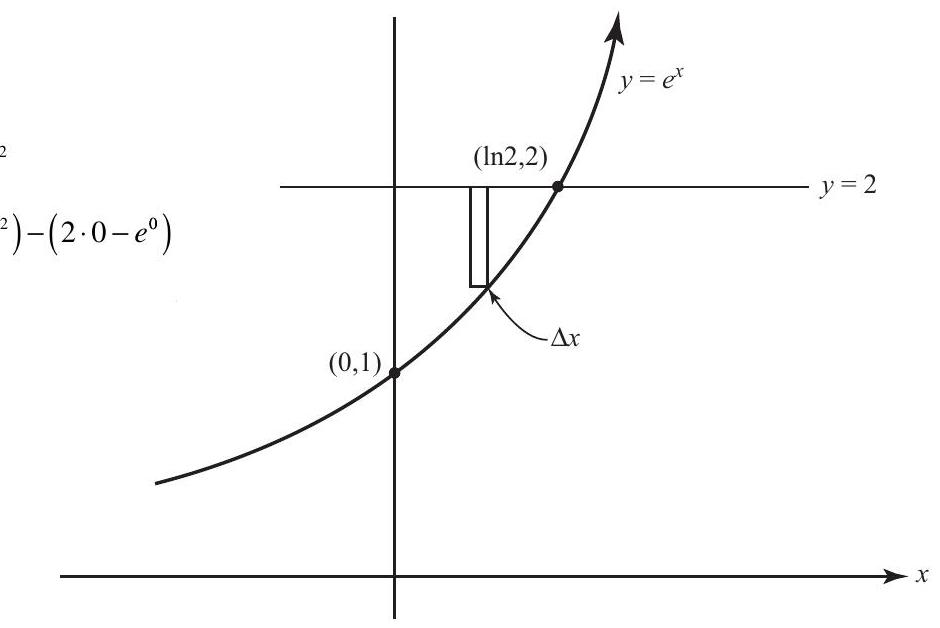
\includegraphics[width=0.50\linewidth]{calculus/images/4dd14383-56bc-4a03-ad67-ca78eb85270b-15_628_940_1994_756.jpg}
\end{center}
\end{solution}




\newpage



\question
The area enclosed by the ellipse with parametric equations $x=2 \cos \theta$ and $y=3 \sin \theta$ equals
\begin{choices}
  \CorrectChoice $6 \pi$
  \choice $\dfrac{9}{2} \pi$
  \choice $3 \pi$
  \choice $\dfrac{3}{2} \pi$
  \choice none of these
\end{choices}
\begin{solution}
(A)\\
\begin{center}
  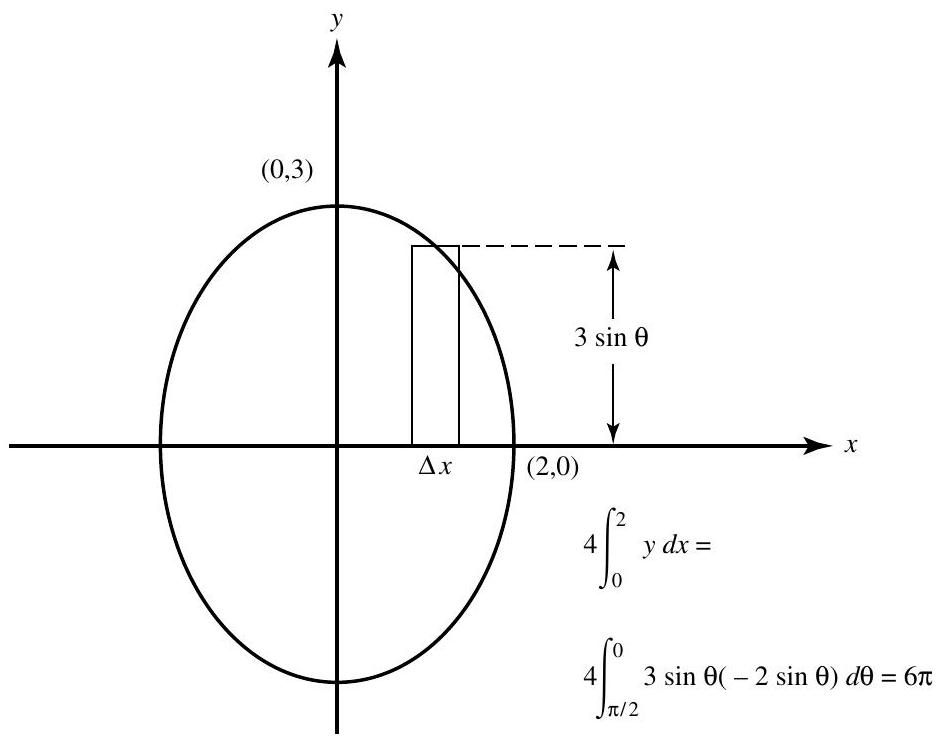
\includegraphics[width=0.50\linewidth]{calculus/images/4dd14383-56bc-4a03-ad67-ca78eb85270b-16_744_945_310_835.jpg}
\end{center}
\end{solution}

\question
The area enclosed by one arch of the cycloid with parametric equations $x=\theta-\sin \theta$ and $y=1-\cos \theta$ equals
\begin{choices}
  \choice $\dfrac{3 \pi}{2}$
  \CorrectChoice $3 \pi$
  \choice $2 \pi$
  \choice $6 \pi$
  \choice none of these
\end{choices}
\begin{solution}
(B)\\
\begin{center}
  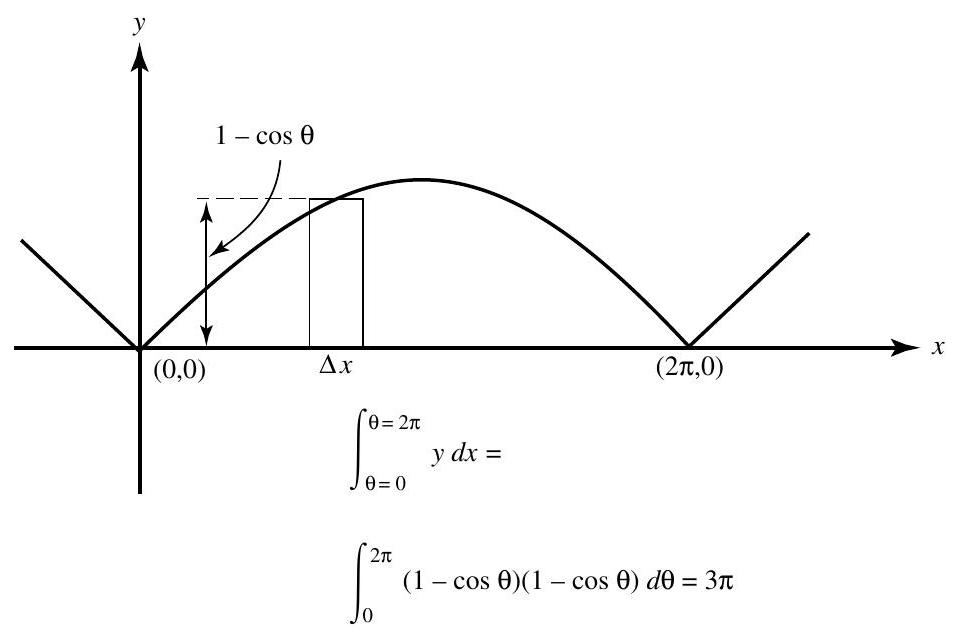
\includegraphics[width=0.50\linewidth]{calculus/images/4dd14383-56bc-4a03-ad67-ca78eb85270b-16_639_957_1136_774.jpg}
\end{center}
\end{solution}



\newpage




\question
The area enclosed by the curve $y^{2}=x(1-x)$ is given by
\begin{choices}
  \choice $2 \int_{0}^{1} x \sqrt{1-x} d x$
  \CorrectChoice $2 \int_{0}^{1} \sqrt{x-x^{2}} d x$
  \choice $4 \int_{0}^{1} \sqrt{x-x^{2}} d x$
  \choice $\pi$
  \choice $2 \pi$
\end{choices}
\begin{solution}
(B)\\
\begin{center}
  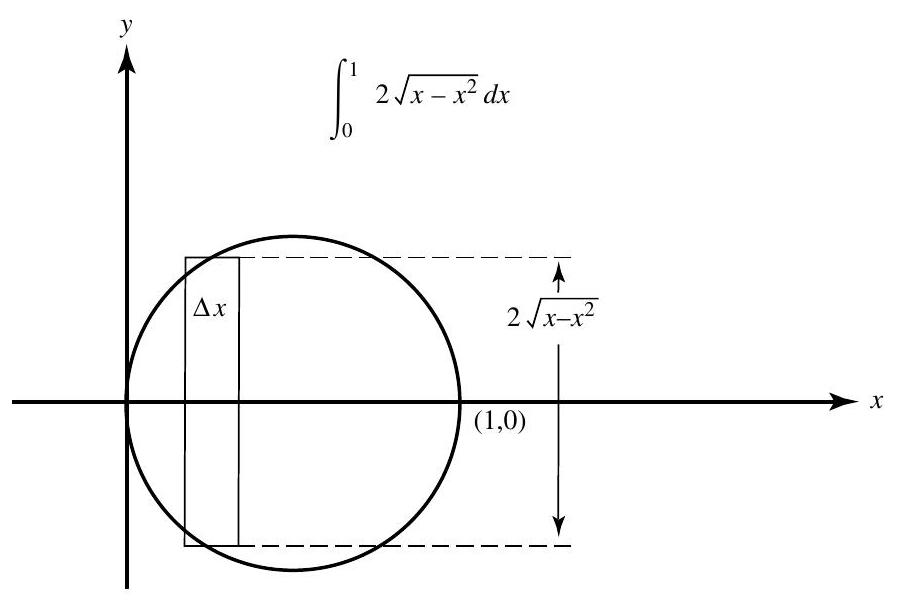
\includegraphics[width=0.50\linewidth]{calculus/images/4dd14383-56bc-4a03-ad67-ca78eb85270b-16_602_899_1846_964.jpg}
\end{center}
\end{solution}




\newpage



\question
The figure below shows part of the curve of $y=x^{3}$ and a rectangle with two vertices at $(0,0)$ and $(c, 0)$. What is the ratio of the area of the rectangle to the shaded part of it above the cubic?
\begin{center}
  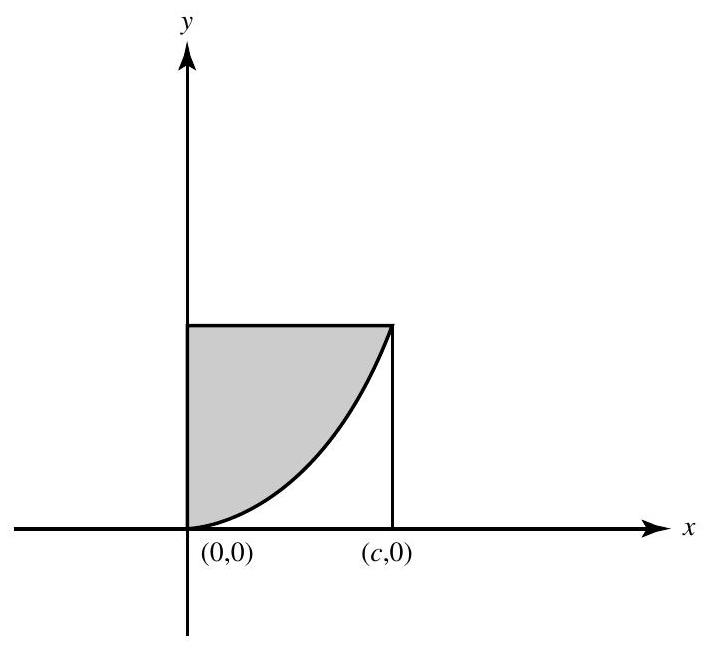
\includegraphics[width=0.50\linewidth]{calculus/images/4dd14383-56bc-4a03-ad67-ca78eb85270b-03_648_711_454_633.jpg}
\end{center}
\begin{choices}
  \choice $3: 4$
  \choice $5: 4$
  \CorrectChoice $4: 3$
  \choice $3: 1$
  \choice $2: 1$
\end{choices}
\begin{solution}
(C)\\
\begin{center}
  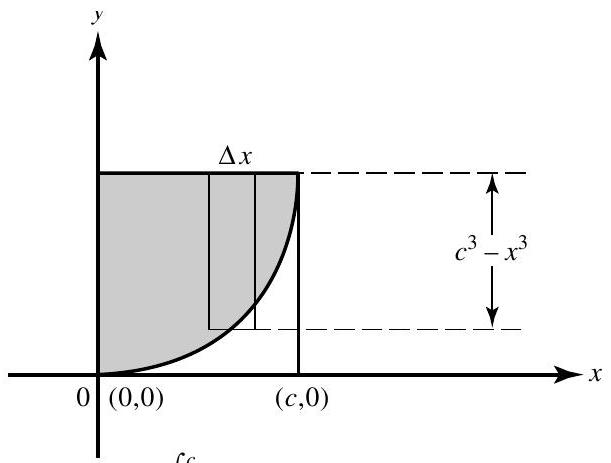
\includegraphics[width=0.50\linewidth]{calculus/images/4dd14383-56bc-4a03-ad67-ca78eb85270b-17_463_611_296_589.jpg}
\end{center}
\[
\begin{aligned}
& \int_{0}^{c}\left(c^{3}-x^{3}\right) d x=\dfrac{3}{4} c^{4} ; \text { thus area of rectangle is to } \\
& \text { area of shaded region as } 4 \text { is to } 3 .
\end{aligned}
\]
\end{solution}




\newpage



\begin{EnvFullwidth}
\textit{In Questions~\ref{calc07:volume-first}--\ref{calc07:volume-last}, the region whose boundaries are given is rotated about the line indicated. Choose the alternative that gives the volume of the solid generated.}
\end{EnvFullwidth}

\question\label{calc07:volume-first}
$y=x^{2}, x=2$, and $y=0$; about the $x$-axis.
\begin{choices}
  \choice $\dfrac{64 \pi}{3}$
  \choice $8 \pi$
  \choice $\dfrac{8 \pi}{3}$
  \choice $\dfrac{128 \pi}{5}$
  \CorrectChoice $\dfrac{32 \pi}{5}$
\end{choices}
\begin{solution}
(E)
\begin{center}
  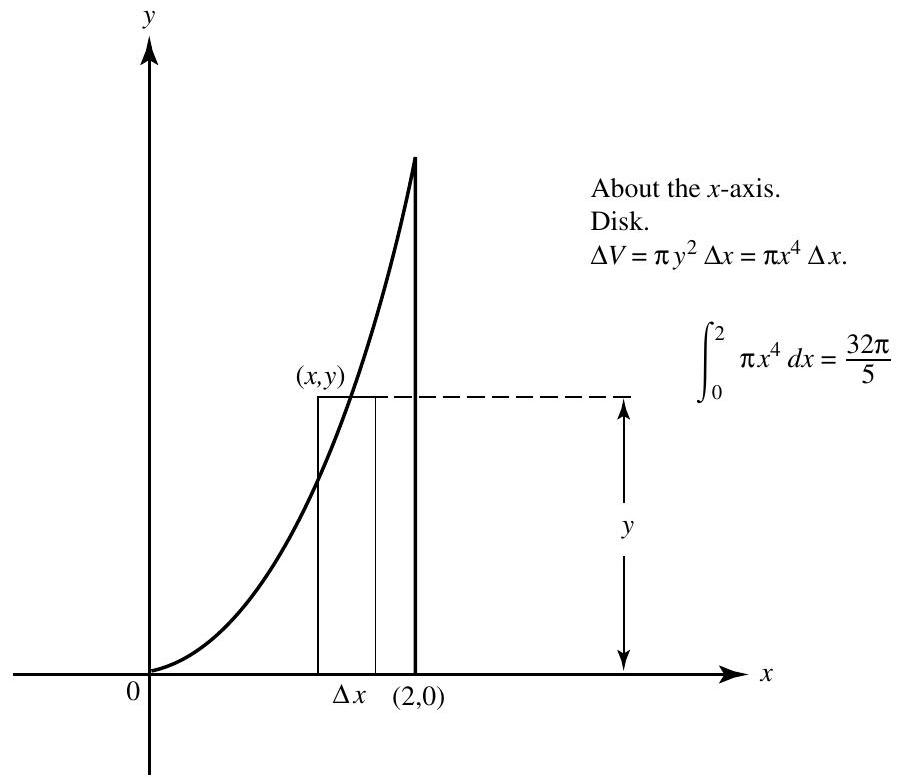
\includegraphics[width=0.50\linewidth]{calculus/images/4dd14383-56bc-4a03-ad67-ca78eb85270b-17_782_901_1127_616.jpg}
\end{center}
\end{solution}




\newpage



\question
$y=x^{2}, x=2$, and $y=0$; about the $y$-axis.
\begin{choices}
  \choice $\dfrac{16 \pi}{3}$
  \choice $4 \pi$
  \choice $\dfrac{32 \pi}{5}$
  \CorrectChoice $8 \pi$
  \choice $\dfrac{8 \pi}{3}$
\end{choices}
\begin{solution}
(D)
\begin{center}
  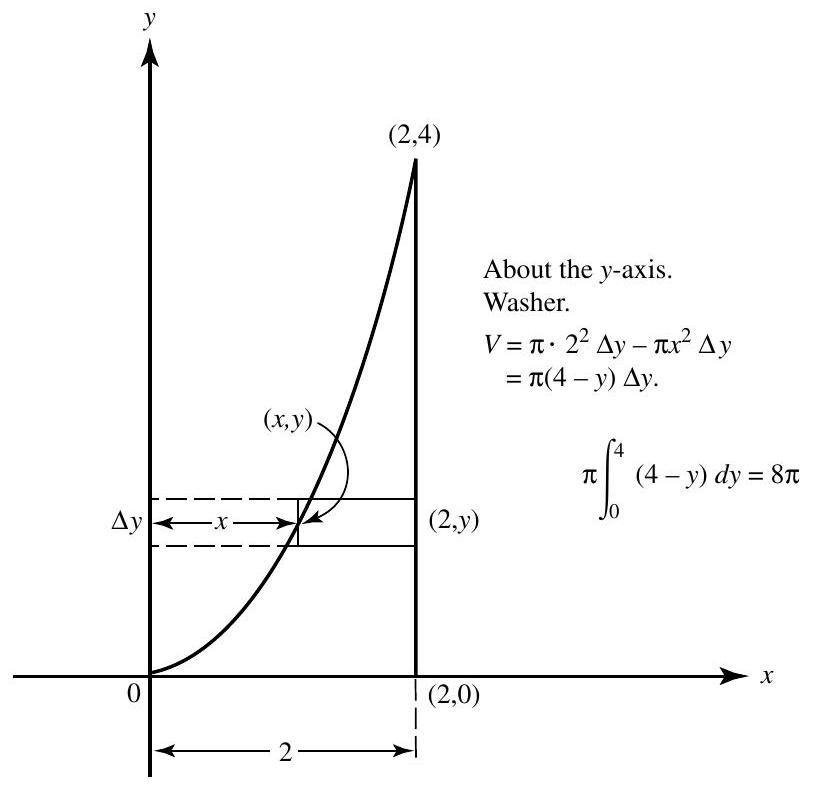
\includegraphics[width=0.50\linewidth]{calculus/images/4dd14383-56bc-4a03-ad67-ca78eb85270b-18_789_813_299_1032.jpg}
\end{center}
\end{solution}

\question
The first quadrant region bounded by $y=x^{2}$, the $y$-axis, and $y=4$; about the $y$-axis.
\begin{choices}
  \CorrectChoice $8 \pi$
  \choice $4 \pi$
  \choice $\dfrac{64 \pi}{3}$
  \choice $\dfrac{32 \pi}{3}$
  \choice $\dfrac{16 \pi}{3}$
\end{choices}
\begin{solution}
(A)

About the $y$-axis. Disk.
$\Delta V=\pi x^{2} \Delta y$
$=\pi y \Delta y$.
$\pi \int_{0}^{4} y d y=8 \pi$
\end{solution}




\newpage



\question
$y=x^{2}$ and $y=4$; about the $x$-axis.
\begin{choices}
  \choice $\dfrac{64 \pi}{5}$
  \choice $\dfrac{512 \pi}{15}$
  \CorrectChoice $\dfrac{256 \pi}{5}$
  \choice $\dfrac{128 \pi}{5}$
  \choice none of these
\end{choices}
\begin{solution}
(C)
\begin{center}
  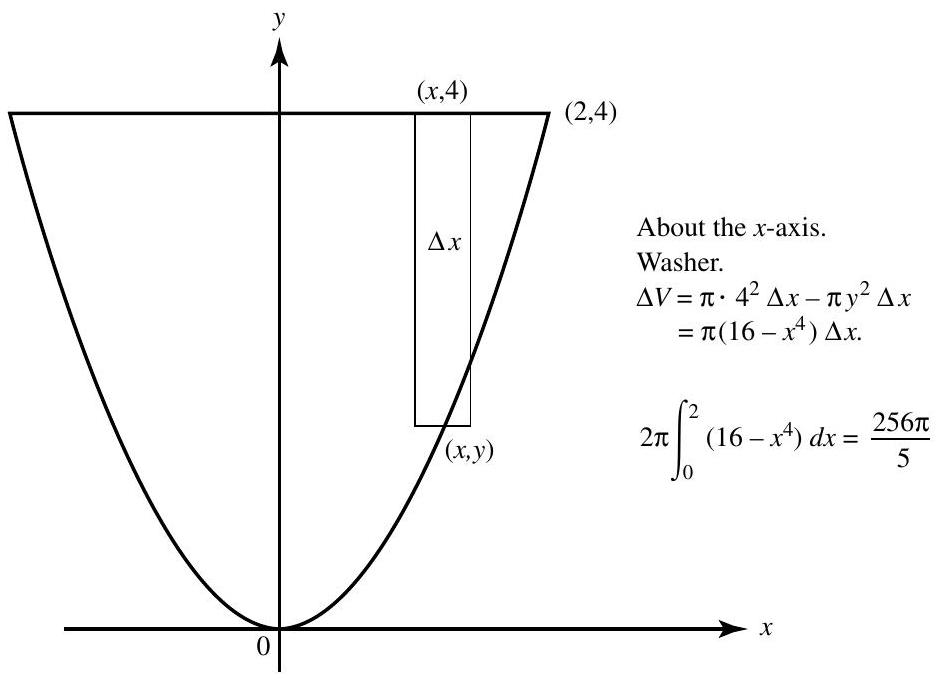
\includegraphics[width=0.50\linewidth]{calculus/images/4dd14383-56bc-4a03-ad67-ca78eb85270b-18_681_945_1878_937.jpg}
\end{center}
\end{solution}




\newpage



\question
$y=x^{2}$ and $y=4$; about the line $y=4$.
\begin{choices}
  \choice $\dfrac{256 \pi}{15}$
  \choice $\dfrac{256 \pi}{5}$
  \choice $\dfrac{512 \pi}{5}$
  \CorrectChoice $\dfrac{512 \pi}{15}$
  \choice $\dfrac{64 \pi}{3}$
\end{choices}
\begin{solution}
(D)
\begin{center}
  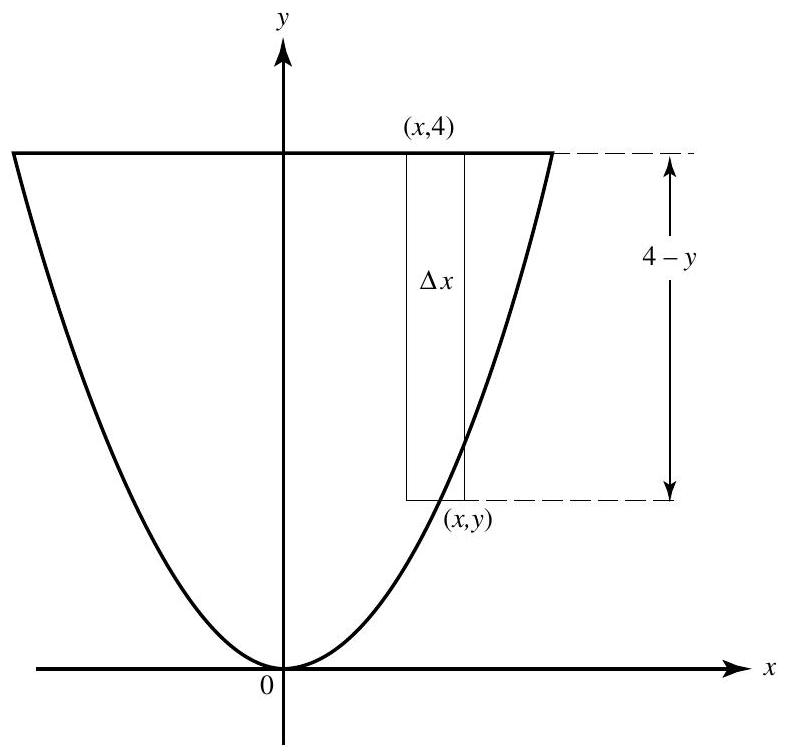
\includegraphics[width=0.50\linewidth]{calculus/images/4dd14383-56bc-4a03-ad67-ca78eb85270b-19_753_787_301_487.jpg}
\end{center}
About $y=4$.\\
Disk.
\[
\begin{aligned}
\Delta V & =\pi(4-y)^{2} \Delta x \\
& =\pi\left(4-x^{2}\right)^{2} \Delta x
\end{aligned}
\]
$2 \pi \int_{0}^{2}\left(4-x^{2}\right)^{2} d x=\dfrac{512 \pi}{15}$
\end{solution}




\newpage



\question
An arch of $y=\sin x$ and the $x$-axis; about the $x$-axis.
\begin{choices}
  \choice $\dfrac{\pi}{2}\left(\pi-\dfrac{1}{2}\right)$
  \CorrectChoice $\dfrac{\pi^{2}}{2}$
  \choice $\dfrac{\pi^{2}}{4}$
  \choice $\pi^{2}$
  \choice $\pi(\pi-1)$
\end{choices}
\begin{solution}
(B)
\begin{center}
  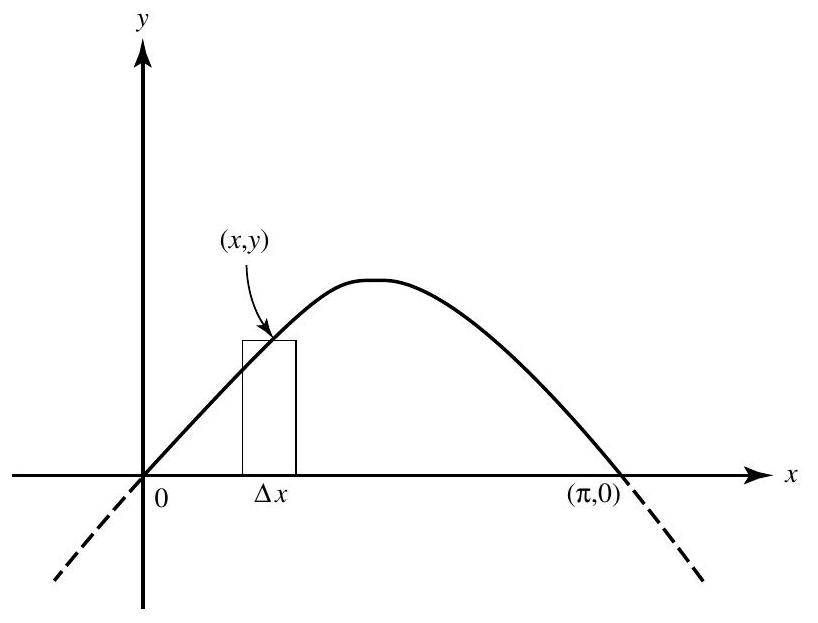
\includegraphics[width=0.50\linewidth]{calculus/images/4dd14383-56bc-4a03-ad67-ca78eb85270b-19_623_818_1099_454.jpg}
\end{center}
About the $x$-axis.\\
Disk.
\[
\begin{aligned}
\Delta V & =\pi y^{2} \Delta x \\
& =\pi \sin ^{2} x \Delta x
\end{aligned}
\]
$\pi \int_{0}^{\pi} \sin ^{2} x d x=\dfrac{\pi^{2}}{2}$
\end{solution}




\newpage



\question
A trapezoid with vertices at $(2,0),(2,2),(4,0)$, and $(4,4)$; about the $x$-axis.
\begin{choices}
  \CorrectChoice $\dfrac{56 \pi}{3}$
  \choice $\dfrac{128 \pi}{3}$
  \choice $\dfrac{92 \pi}{3}$
  \choice $\dfrac{112 \pi}{3}$
  \choice none of these
\end{choices}
\begin{solution}
(A)
\begin{center}
  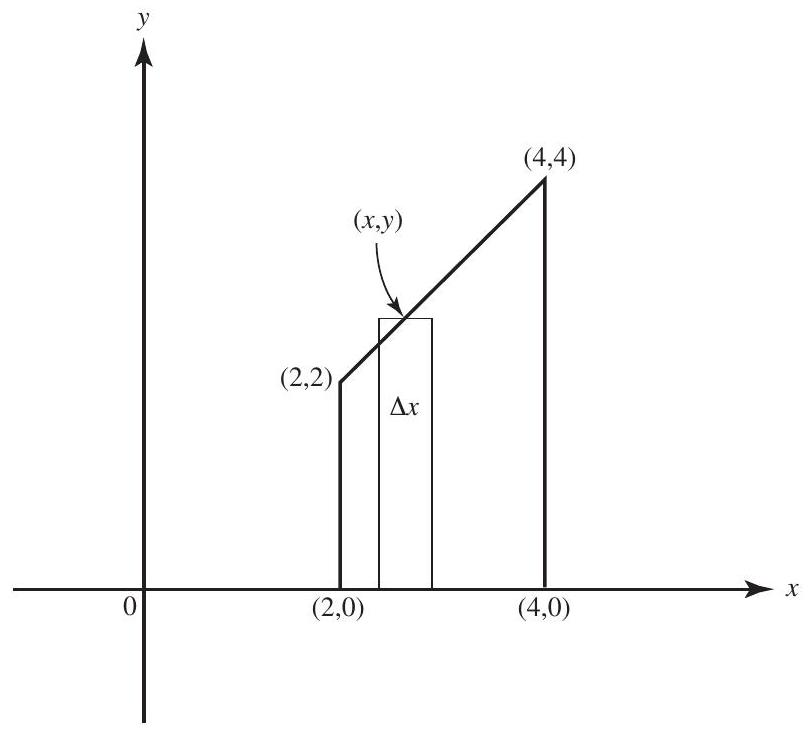
\includegraphics[width=0.50\linewidth]{calculus/images/4dd14383-56bc-4a03-ad67-ca78eb85270b-19_732_811_1850_461.jpg}
\end{center}
About the $x$-axis.\\
Disk.
$\Delta V=\pi y^{2} \Delta x$
$\pi \int_{2}^{4} x^{2} d x=\dfrac{56 \pi}{3}$
\end{solution}




\newpage



\question
The base of a solid is a circle of radius $a$, and every plane section perpendicular to a diameter is a square. The solid has volume
\begin{choices}
  \choice $\dfrac{8}{3} a^{3}$
  \choice $2 \pi a^{3}$
  \choice $4 \pi a^{3}$
  \CorrectChoice $\dfrac{16}{3} a^{3}$
  \choice $\dfrac{8 \pi}{3} a^{3}$
\end{choices}
\begin{solution}
\begin{center}
  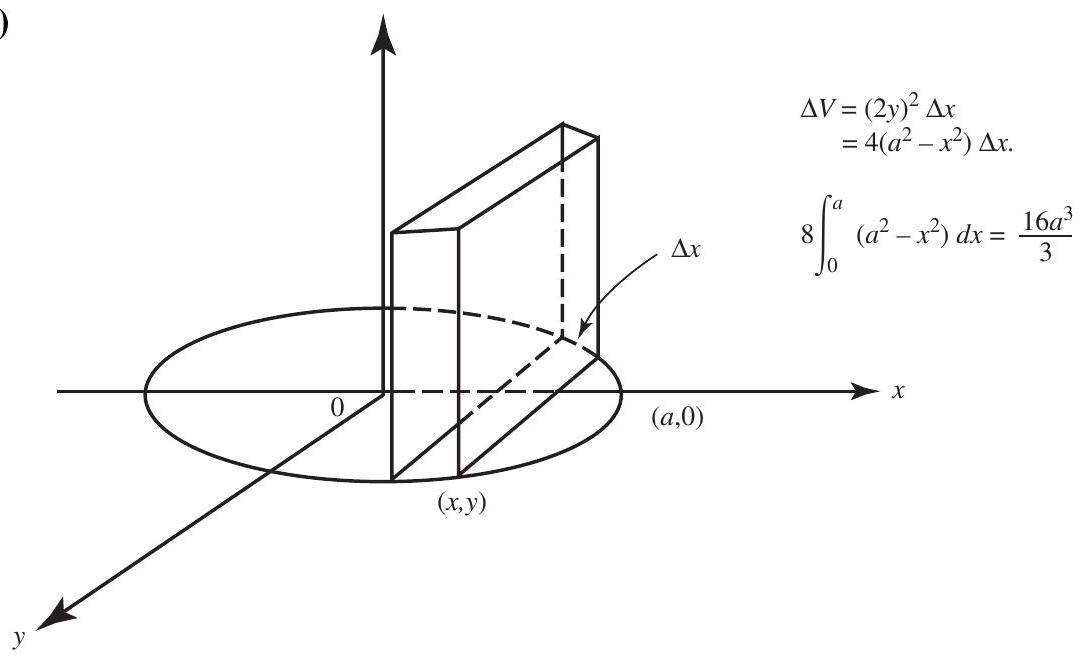
\includegraphics[width=0.50\linewidth]{calculus/images/4dd14383-56bc-4a03-ad67-ca78eb85270b-20_662_1091_296_807.jpg}
\end{center}
\end{solution}

\question
The base of a solid is the region bounded by the parabola $x^{2}=8 y$ and the line $y=4$, and each plane section perpendicular to the $y$-axis is an equilateral triangle. The volume of the solid is
\begin{choices}
  \choice $\dfrac{64 \sqrt{3}}{3}$
  \CorrectChoice $64 \sqrt{3}$
  \choice $32 \sqrt{3}$
  \choice $32$
  \choice none of these
\end{choices}
\begin{solution}
\begin{center}
  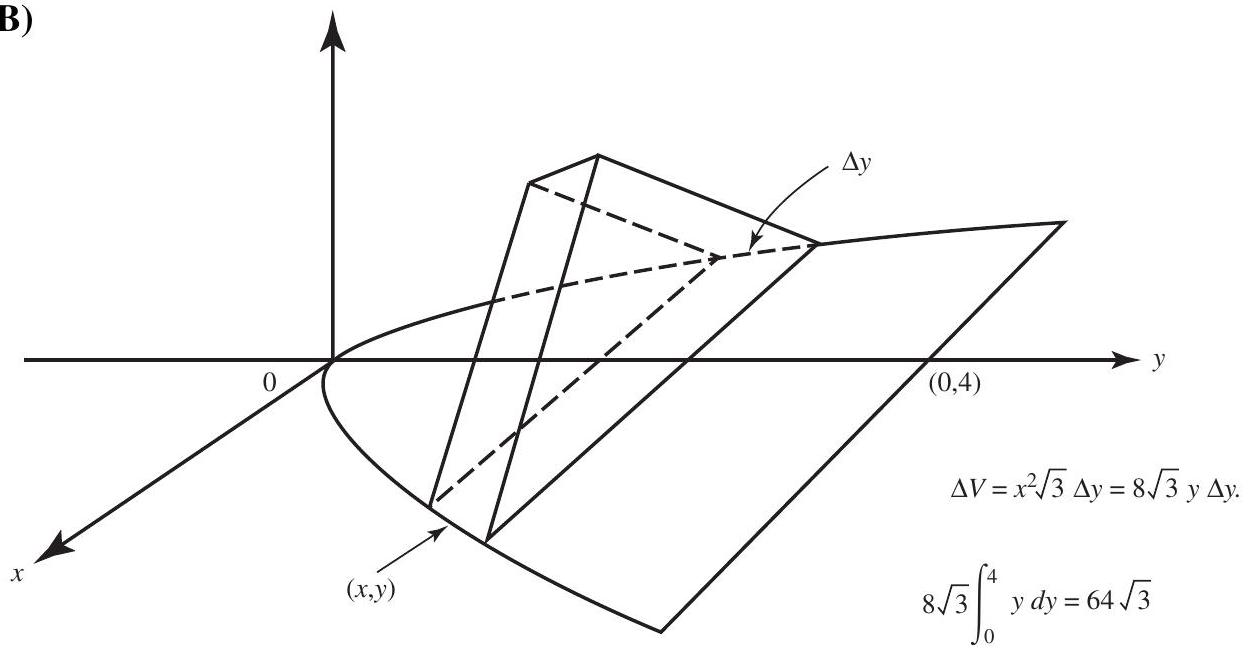
\includegraphics[width=0.50\linewidth]{calculus/images/4dd14383-56bc-4a03-ad67-ca78eb85270b-20_658_1254_1057_781.jpg}
\end{center}
\end{solution}




\newpage



\question\label{calc07:volume-last}
The base of a solid is the region bounded by $y=e^{-x}$, the $x$-axis, the $y$-axis, and the line $x=1$. Each cross section perpendicular to the $x$-axis is a square. The volume of the solid is
\begin{choices}
  \choice $\dfrac{e^{2}}{2}$
  \choice $e^{2}-1$
  \choice $1-\dfrac{1}{e^{2}}$
  \choice $\dfrac{e^{2}-1}{2}$
  \CorrectChoice $\dfrac{1}{2}\left(1-\dfrac{1}{e^{2}}\right)$


\end{choices}
\begin{solution}
\begin{center}
  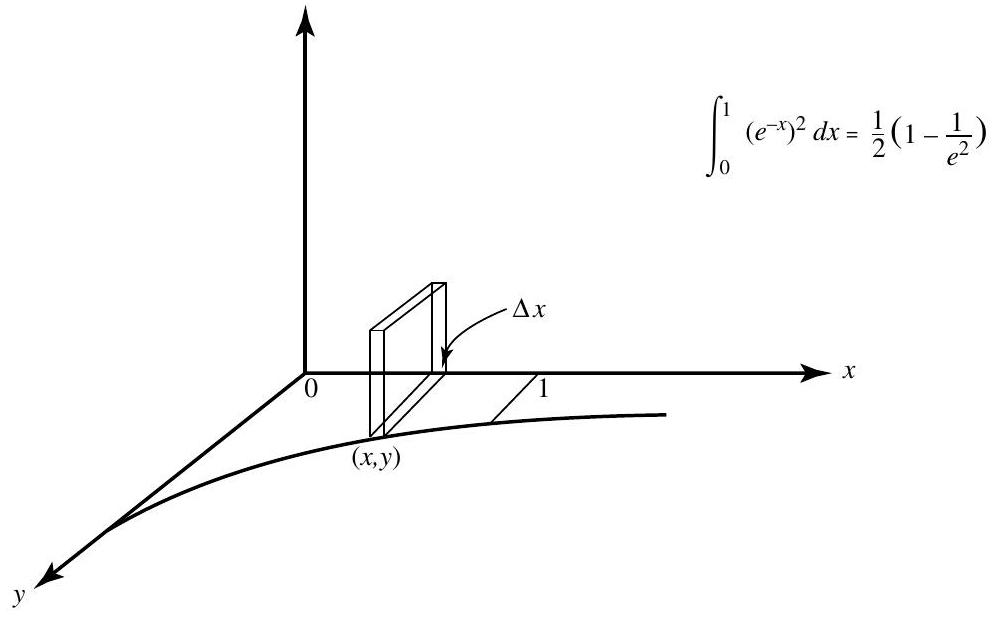
\includegraphics[width=0.50\linewidth]{calculus/images/4dd14383-56bc-4a03-ad67-ca78eb85270b-20_620_996_1837_930.jpg}
\end{center}

\end{solution}

\question
The length of the arc of the curve $y^{2}=x^{3}$ cut off by the line $x=4$ is
\begin{choices}
  \choice $\dfrac{4}{3}(10 \sqrt{10}-1)$
  \choice $\dfrac{8}{27}\left(10^{3 / 2}-1\right)$
  \CorrectChoice $\dfrac{16}{27}\left(10^{3 / 2}-1\right)$
  \choice $\dfrac{16}{27} 10 \sqrt{10}$
  \choice none of these
\end{choices}
\begin{solution}
Note that the curve is symmetric to the $x$-axis. The arc length equals
\[
2 \int_{0}^{4} \sqrt{1+\dfrac{9}{4} x} d x
\]
\end{solution}




\newpage



\question
The length of the arc of $y=\ln \cos x$ from $x=\dfrac{\pi}{4}$ to $x=\dfrac{\pi}{3}$ equals
\begin{choices}
  \CorrectChoice $\ln \dfrac{\sqrt{3}+2}{\sqrt{2}+1}$
  \choice $2$
  \choice $\ln (1+\sqrt{3}-\sqrt{2})$
  \choice $\sqrt{3}-2$
  \choice $\dfrac{\ln (\sqrt{3}+2)}{\ln (\sqrt{2}+1)}$
\end{choices}
\begin{solution}
Integrate $\int_{\pi / 4}^{\pi / 3} \sqrt{1+\tan ^{2} x} d x$. Replace the integrand by $\sec x$, and use formula (13) on page 216 to get $\left.\ln |\sec x+\tan x|\right|_{\pi / 4} ^{\pi / 3}$.



\end{solution}

\question
\[
\int_{0}^{\infty} e^{-x}\,dx=
\]
\begin{choices}
  \CorrectChoice $1$
  \choice $\dfrac{1}{e}$
  \choice $-1$
  \choice $-\dfrac{1}{e}$
  \choice none of these
\end{choices}
\begin{solution}
The integral equals $\lim\limits_{b \to \infty}-\left.\dfrac{1}{e^{x}}\right|_{0} ^{b}=-(0-1)$.
\end{solution}

\question
\[
\int_{0}^{e} \dfrac{d u}{u}=
\]
\begin{choices}
  \choice $1$
  \choice $\dfrac{1}{e}$
  \choice $-\dfrac{1}{e^{2}}$
  \choice $-1$
  \CorrectChoice none of these
\end{choices}
\begin{solution}
$\int_{0}^{e} \dfrac{d u}{u}=\lim\limits_{h \to 0^{+}} \int_{h}^{e} \dfrac{d u}{u}=\left.\lim\limits_{h \to 0^{+}} \ln |u|\right|_{h} ^{e}=\lim\limits_{h \to 0^{+}}(\ln e-\ln h)$. So the integral diverges to infinity.
\end{solution}




\newpage



\question
\[
\int_{1}^{2} \dfrac{d t}{\sqrt[3]{t-1}}=
\]
\begin{choices}
  \choice $\dfrac{2}{3}$
  \CorrectChoice $\dfrac{3}{2}$
  \choice $3$
  \choice $1$
  \choice none of these
\end{choices}
\begin{solution}
Redefine as $\lim\limits_{k \to 1^{+}} \int_{k}^{2}(t-1)^{-1 / 3} d t$.
\end{solution}

\question
\[
\int_{2}^{4} \dfrac{d x}{(x-3)^{2 / 3}}=
\]
\begin{choices}
  \CorrectChoice $6$
  \choice $\dfrac{6}{5}$
  \choice $\dfrac{2}{3}$
  \choice $0$
  \choice none of these
\end{choices}
\begin{solution}
Rewrite as $\lim\limits_{k \to 3^{-}} \int_{2}^{k}(x-3)^{-2 / 3} d x+\lim\limits_{m \to 3^{+}} \int_{m}^{4}(x-3)^{-2 / 3} d x$. Each integral converges to 3 .
\end{solution}

\question
\[
\int_{2}^{4} \dfrac{d x}{(x-3)^{2}}=
\]
\begin{choices}
  \choice $2$
  \choice $-2$
  \choice $0$
  \choice $\dfrac{2}{3}$
  \CorrectChoice none of these
\end{choices}
\begin{solution}
$\int_{2}^{4} \dfrac{d x}{(x-3)^{2}}=\int_{2}^{3} \dfrac{d x}{(x-3)^{2}}+\int_{3}^{4} \dfrac{d x}{(x-3)^{2}}$. Neither of the latter integrals converges; therefore the original integral diverges.
\end{solution}




\newpage



\question
\[
\int_{0}^{\pi / 2} \dfrac{\sin x}{\sqrt{1-\cos x}}\,dx
\]
\begin{choices}
  \choice $-2$
  \choice $\dfrac{2}{3}$
  \CorrectChoice $2$
  \choice $\dfrac{1}{2}$
  \choice none of these
\end{choices}
\begin{solution}
Evaluate $\left.\lim\limits_{k \to(\pi / 2)^{-}} 2 \sqrt{1-\cos x}\right|_{0} ^{k}$.
\end{solution}

\begin{EnvFullwidth}
\textit{In Questions~\ref{calc07:improper-area-first}--\ref{calc07:improper-area-last}, choose the alternative that gives the area, if it exists, of the region described.}
\end{EnvFullwidth}

\question\label{calc07:improper-area-first}
In the first quadrant under the curve of $y=e^{-x}$.
\begin{choices}
  \CorrectChoice $1$
  \choice $e$
  \choice $\dfrac{1}{e}$
  \choice $2$
  \choice none of these
\end{choices}
\begin{solution}
\begin{center}
  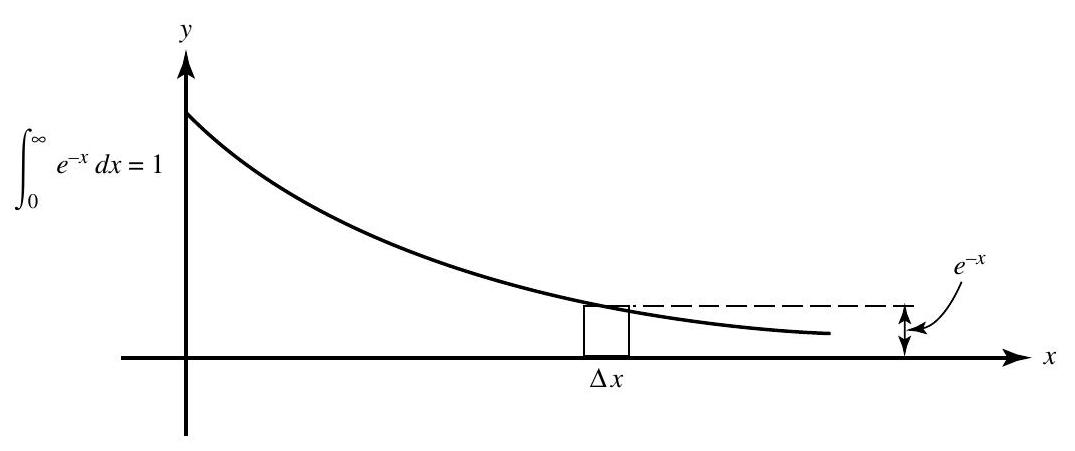
\includegraphics[width=0.50\linewidth]{calculus/images/4dd14383-56bc-4a03-ad67-ca78eb85270b-21_451_1075_1878_470.jpg}
\end{center}
\end{solution}




\newpage



\question
In the first quadrant under the curve of $y=x e^{-x^{2}}$.
\begin{choices}
  \choice $2$
  \choice $\dfrac{2}{e}$
  \CorrectChoice $\dfrac{1}{2}$
  \choice $\dfrac{1}{2 e}$
  \choice none of these
\end{choices}
\begin{solution}
\begin{center}
  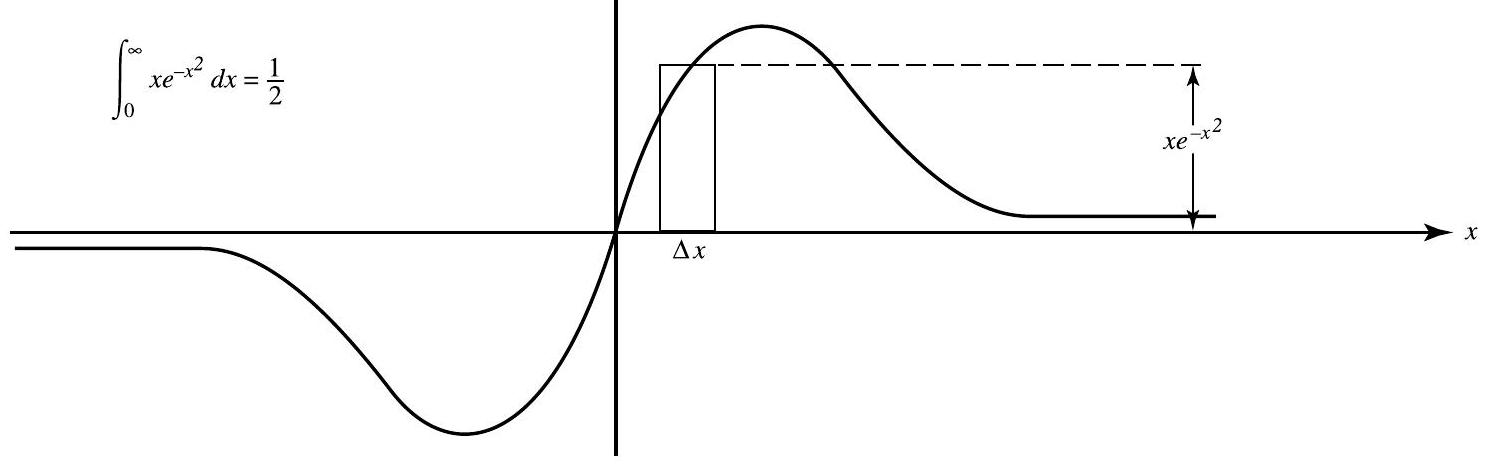
\includegraphics[width=0.50\linewidth]{calculus/images/4dd14383-56bc-4a03-ad67-ca78eb85270b-22_468_1488_411_546.jpg}
\end{center}
\end{solution}

\question
In the first quadrant above $y=1$, between by the $y$-axis and the curve $x y=1$.
\begin{choices}
  \choice $1$
  \choice $2$
  \choice $\dfrac{1}{2}$
  \choice $4$
  \CorrectChoice none of these
\end{choices}
\begin{solution}
\begin{center}
  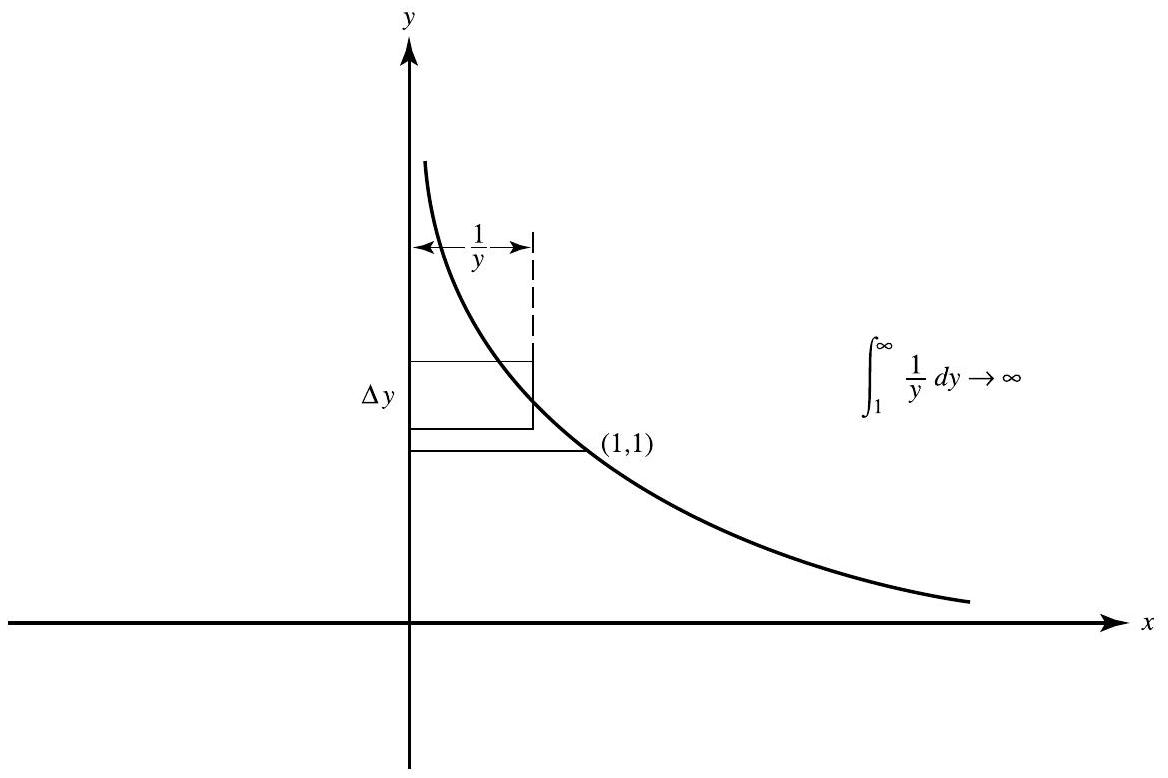
\includegraphics[width=0.50\linewidth]{calculus/images/4dd14383-56bc-4a03-ad67-ca78eb85270b-22_778_1168_937_825.jpg}
\end{center}
\end{solution}




\newpage



\question
Between the curve $y=\dfrac{4}{1+x^{2}}$ and the $x$-axis.
\begin{choices}
  \choice $2 \pi$
  \CorrectChoice $4 \pi$
  \choice $8 \pi$
  \choice $\pi$
  \choice none of these
\end{choices}
\begin{solution}
\begin{center}
  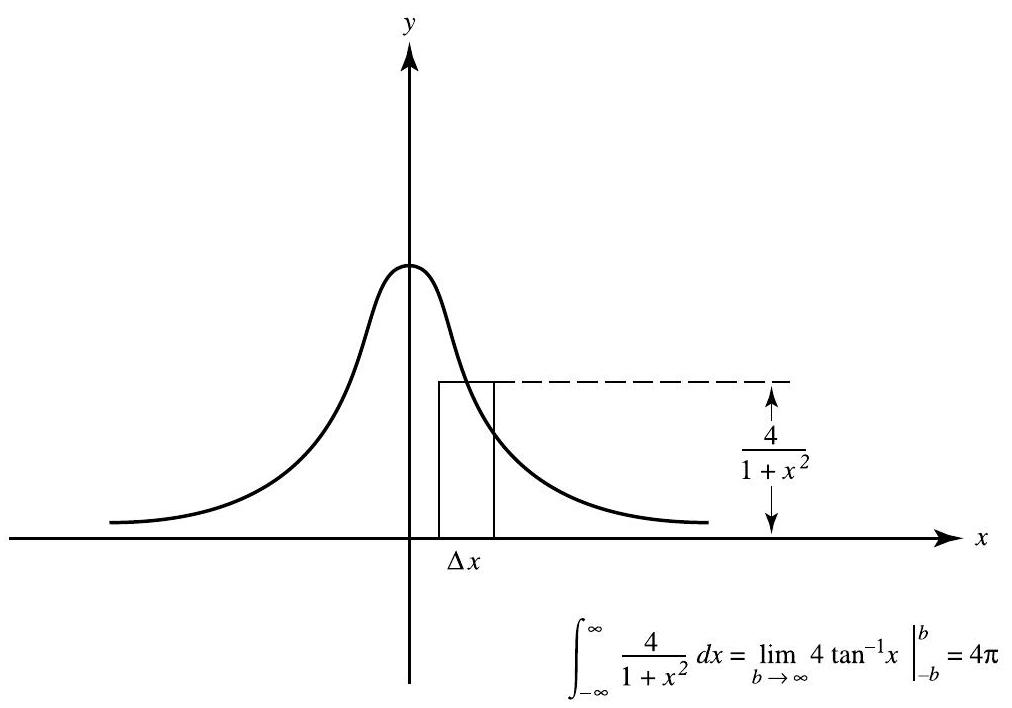
\includegraphics[width=0.50\linewidth]{calculus/images/4dd14383-56bc-4a03-ad67-ca78eb85270b-22_708_1012_1730_828.jpg}
\end{center}
\end{solution}


\newpage



\question\label{calc07:improper-area-last}
Above the $x$-axis, between the curve $y=\dfrac{4}{\sqrt{1-x^{2}}}$ and its asymptotes.
\begin{choices}
  \choice $\dfrac{\pi}{2}$
  \choice $\pi$
  \choice $2 \pi$
  \CorrectChoice $4 \pi$
  \choice none of these
\end{choices}
\begin{solution}
\begin{center}
  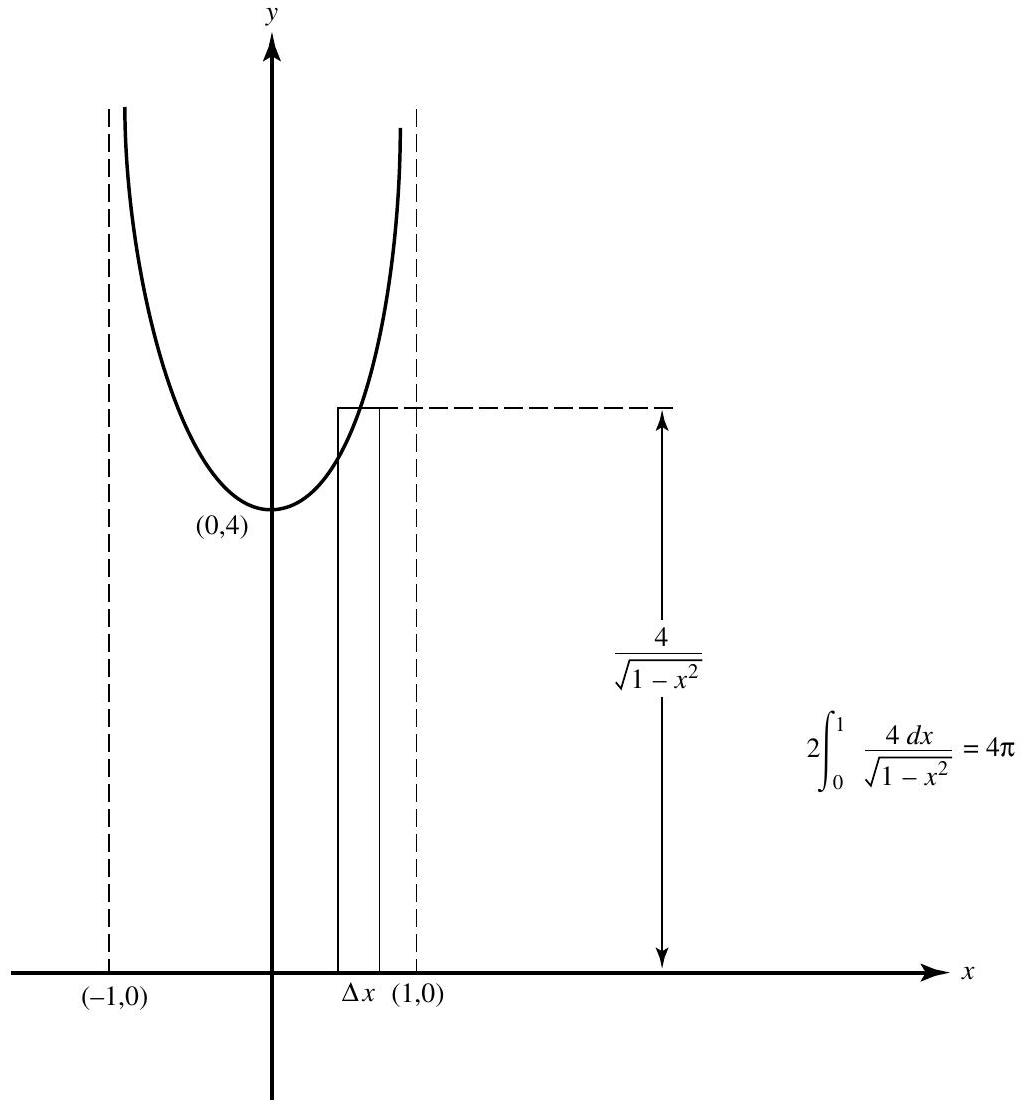
\includegraphics[width=0.50\linewidth]{calculus/images/4dd14383-56bc-4a03-ad67-ca78eb85270b-23_1107_1028_320_538.jpg}
\end{center}
\end{solution}

\newpage


\begin{EnvFullwidth}
\textit{In Questions~\ref{calc07:improper-vol-first} and~\ref{calc07:improper-vol-last}, choose the alternative that gives the volume, if it exists, of the solid generated.}
\end{EnvFullwidth}

\question\label{calc07:improper-vol-first}
$y=\dfrac{1}{x}$, at the left by $x=1$, and below by $y=0$; about the $x$-axis.
\begin{choices}
  \choice $\dfrac{\pi}{2}$
  \CorrectChoice $\pi$
  \choice $2 \pi$
  \choice $4 \pi$
  \choice none of these
\end{choices}
\begin{solution}
  \begin{center}
    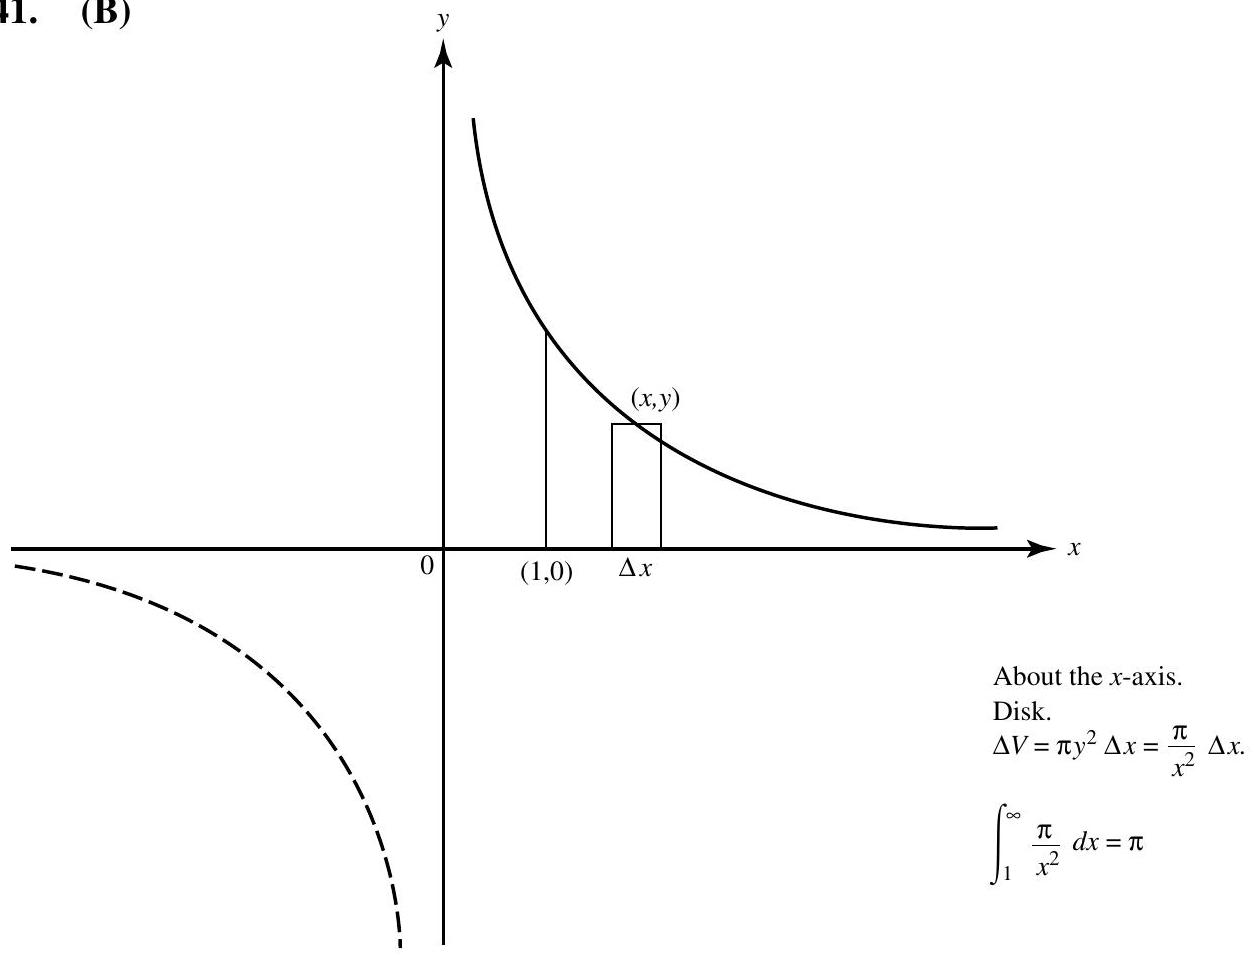
\includegraphics[width=0.50\linewidth]{calculus/images/4dd14383-56bc-4a03-ad67-ca78eb85270b-23_961_1256_1454_317.jpg}
  \end{center}
\end{solution}

\question\label{calc07:improper-vol-last}
The first-quadrant region under $y=e^{-x}$; about the $x$-axis.
\begin{choices}
  \CorrectChoice $\dfrac{\pi}{2}$
  \choice $\pi$
  \choice $2 \pi$
  \choice $4 \pi$
  \choice none of these
\end{choices}
\begin{solution}
  \begin{center}
    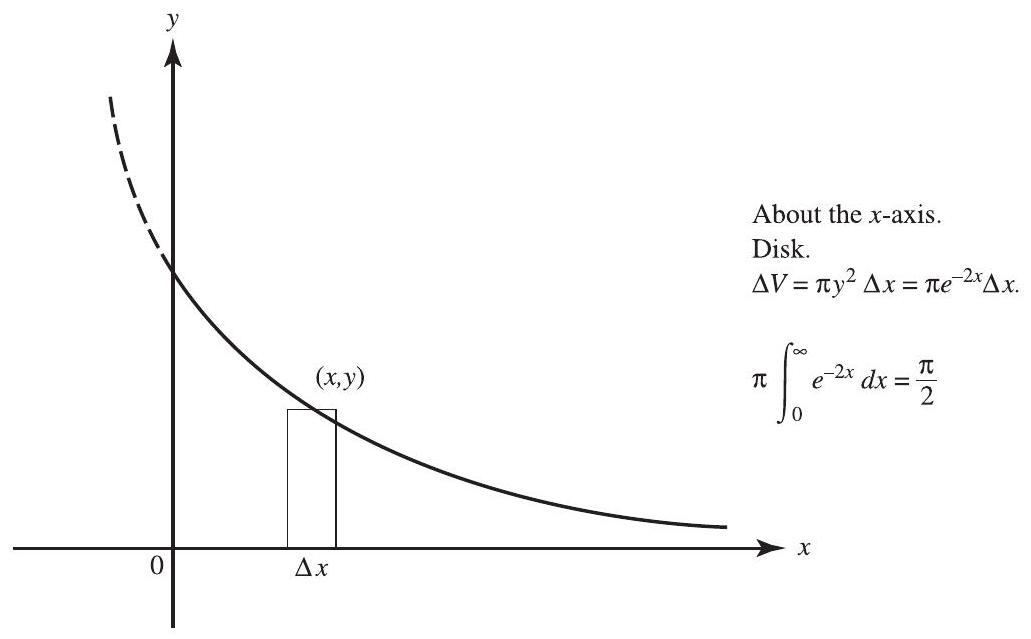
\includegraphics[width=0.50\linewidth]{calculus/images/4dd14383-56bc-4a03-ad67-ca78eb85270b-24_639_1031_301_927.jpg}
  \end{center}
\end{solution}


\newpage


\question
The area bounded by the parabola $y=2-x^{2}$ and the line $y=x-4$ is given by
\begin{center}
  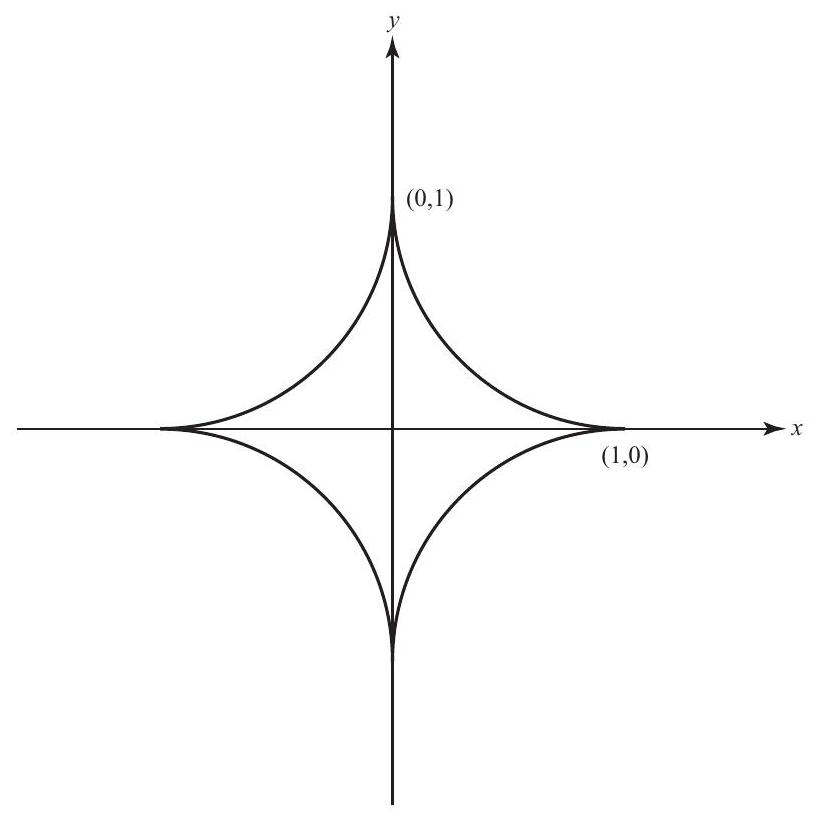
\includegraphics[width=0.50\linewidth]{calculus/images/4dd14383-56bc-4a03-ad67-ca78eb85270b-07_820_819_932_582.jpg}
\end{center}
\begin{choices}
  \choice $\int_{-2}^{3}\left(6-x-x^{2}\right) d x$
  \choice $\int_{-2}^{1}\left(2+x+x^{2}\right) d x$
  \CorrectChoice $\int_{-3}^{2}\left(6-x-x^{2}\right) d x$
  \choice $2 \int_{0}^{\sqrt{2}}\left(2-x^{2}\right) d x+\int_{-3}^{2}(4-x) d x$
  \choice none of these
\end{choices}
\begin{solution}
  \begin{center}
    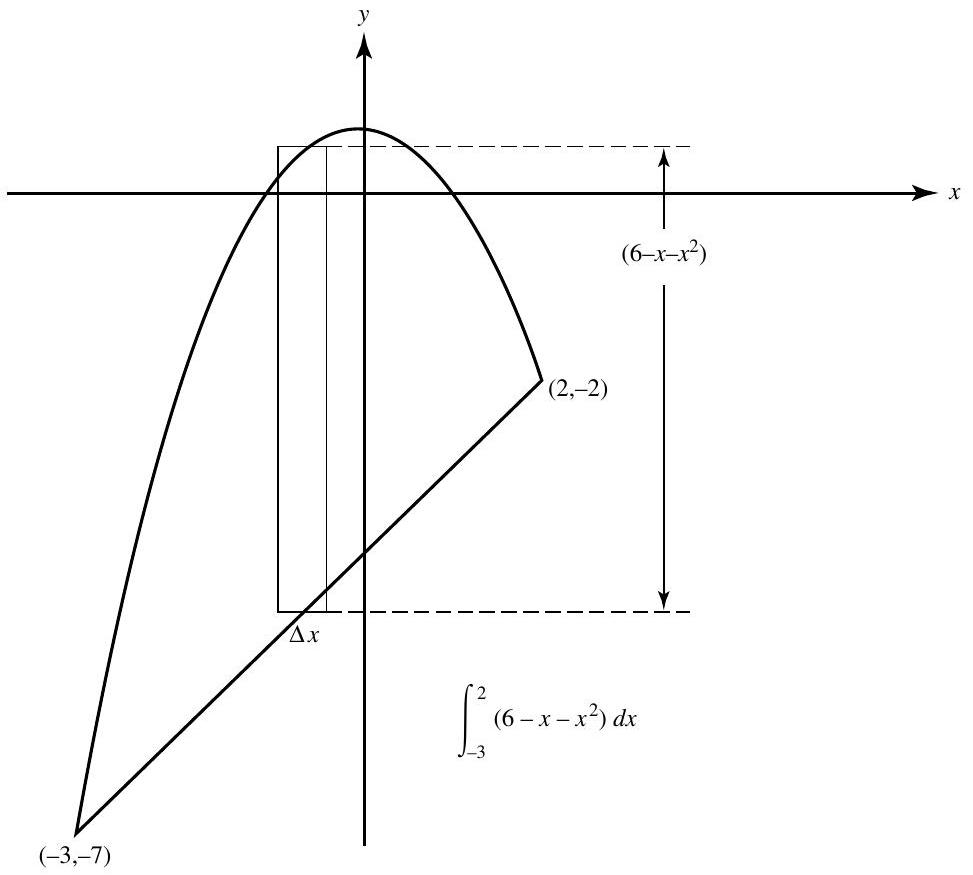
\includegraphics[width=0.50\linewidth]{calculus/images/4dd14383-56bc-4a03-ad67-ca78eb85270b-24_875_973_1062_904.jpg}
  \end{center}
\end{solution}

\newpage

\question
The area enclosed by the hypocycloid with parametric equations $x=\cos ^{3} t$ and $y=\sin ^{3} t$ as shown in the above diagram is
\begin{choices}
  \choice $3 \int_{\pi / 2}^{0} \sin ^{4} t \cos ^{2} t d t$
  \choice $4 \int_{0}^{1} \sin ^{3} t d t$
  \choice $-4 \int_{\pi / 2}^{0} \sin ^{6} t d t$
  \CorrectChoice $12 \int_{0}^{\pi / 2} \sin ^{4} t \cos ^{2} t d t$
  \choice none of these
\end{choices}
\begin{solution}
(D) Use parametric area formula with symmetry.
\begin{center}
  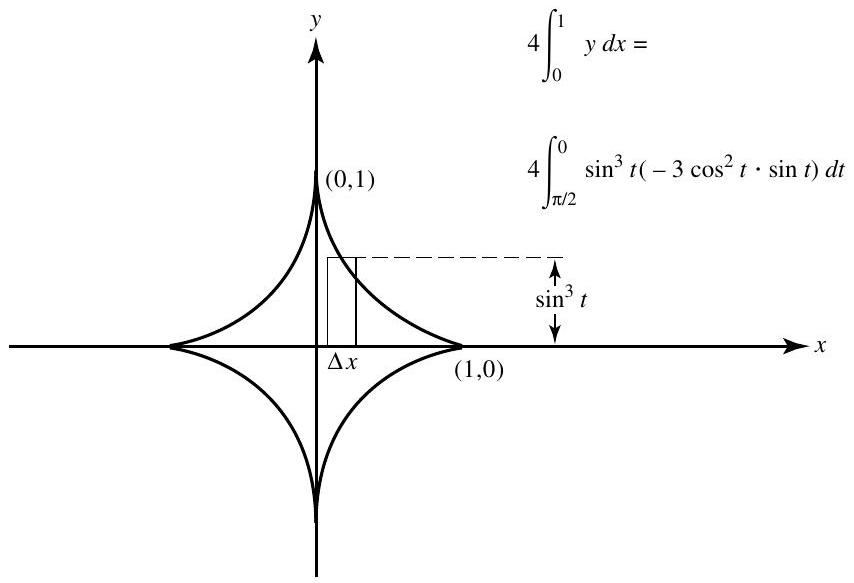
\includegraphics[width=0.50\linewidth]{calculus/images/4dd14383-56bc-4a03-ad67-ca78eb85270b-24_583_854_1994_960.jpg}
\end{center}
\end{solution}

\question
Suppose the following is a table of ordinates for $y=f(x)$, given that $f$ is continuous on $[1,5]$ :

\begin{center}
\begin{tabular}{c|ccccc}
$x$ & 1 & 2 & 3 & 4 & 5 \\
\hline
$y$ & 1.62 & 4.15 & 7.5 & 9.0 & 12.13 \\
\end{tabular}
\end{center}

If a trapezoid sum in used, with $n=4$, then the area under the curve, from $x=1$ to $x=5$, is equal, to two decimal places, to
\begin{choices}
  \choice $6.88$
  \choice $13.76$
  \choice $20.30$
  \choice $25.73$
  \CorrectChoice $27.53$
\end{choices}
\begin{solution}
$T(4)=\dfrac{1}{4}(1.62+2(4.15)+2(7.5)+2(9.0)+12.13)$.
\end{solution}

\newpage


\question
The area $A$ enclosed by the four-leaved rose $r=\cos 2 \theta$ equals, to three decimal places,
\begin{choices}
  \choice $0.785$
  \CorrectChoice $1.571$
  \choice $2.071$
  \choice $3.142$
  \choice $6.283$
\end{choices}
\begin{solution}
$A=8 \int_{0}^{\pi / 4} \dfrac{1}{2} \cos ^{2} 2 \theta d \theta=1.571$, using a graphing calculator.
\end{solution}

\question
The area bounded by the small loop of the limaon $r=1-2 \sin \theta$ is given by the definite integral
\begin{choices}
  \choice $\int_{\pi / 3}^{5 \pi / 3}\left[\dfrac{1}{2}(1-2 \sin \theta)\right]^{2} d \theta$
  \choice $\int_{7 \pi / 6}^{3 \pi / 2}(1-2 \sin \theta)^{2} d \theta$
  \CorrectChoice $\int_{\pi / 6}^{\pi / 2}(1-2 \sin \theta)^{2} d \theta$
  \choice $\int_{0}^{\pi / 6}\left[\dfrac{1}{2}(1-2 \sin \theta)\right]^{2} d \theta+\int_{5 \pi / 6}^{\pi}\left[\dfrac{1}{2}(1-2 \sin \theta)\right]^{2} d \theta$
  \choice $\int_{0}^{\pi / 3}(1-2 \sin \theta)^{2} d \theta$
\end{choices}
\begin{solution}
(C) The small loop is generated as $\theta$ varies from $\dfrac{\pi}{6}$ to $\dfrac{5 \pi}{6}$.
\end{solution}

\newpage


\begin{EnvFullwidth}
\textit{In Questions~\ref{calc07:volume2-first}--\ref{calc07:volume2-last}, the region whose boundaries are given is rotated about the line indicated. Choose the alternative that gives the volume of the solid generated.}
\end{EnvFullwidth}

\question\label{calc07:volume2-first}
$y=x^{2}$ and $y=4$; about the line $y=-1$.
\begin{choices}
  \choice $4 \pi \int_{-1}^{4}(y+1) \sqrt{y} d y$
  \choice $2 \pi \int_{0}^{2}\left(4-x^{2}\right)^{2} d x$
  \choice $\pi \int_{-2}^{2}\left(16-x^{4}\right) d x$
  \CorrectChoice $2 \pi \int_{0}^{2}\left(24-2 x^{2}-x^{4}\right) d x$
  \choice none of these
\end{choices}
\begin{solution}
(D)
\begin{center}
  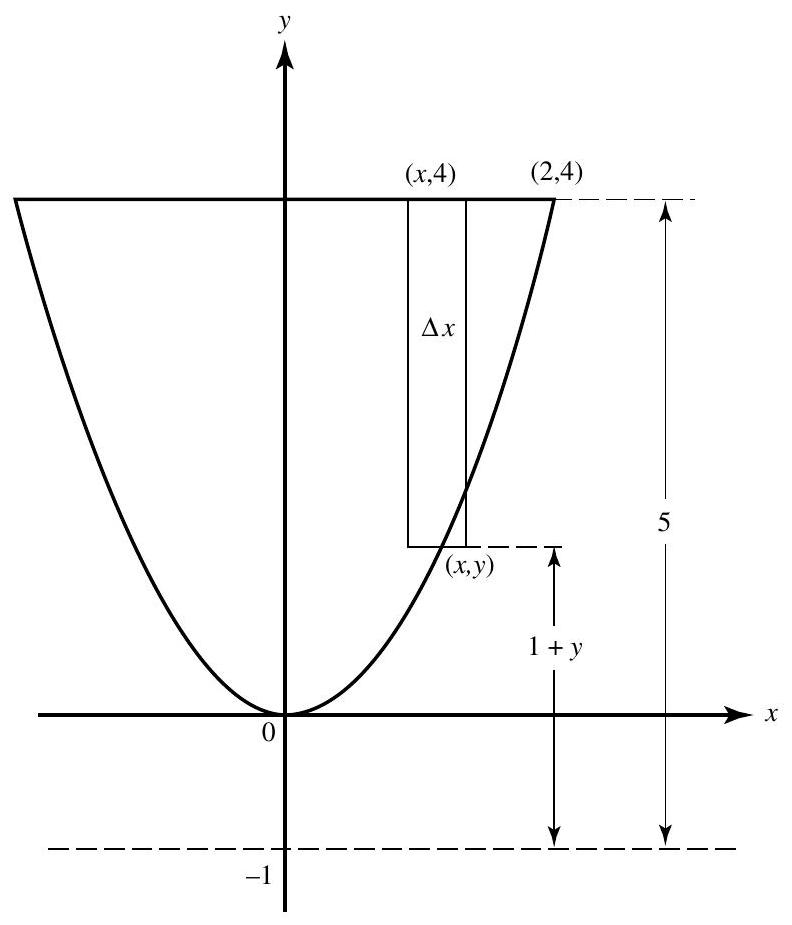
\includegraphics[width=0.50\linewidth]{calculus/images/4dd14383-56bc-4a03-ad67-ca78eb85270b-25_925_792_841_487.jpg}
\end{center}
About $y=-1$.\\
Washer.
\[
\begin{aligned}
\Delta V & =\pi \cdot 5^{2} \Delta x-\pi(1+y)^{2} \Delta x \\
& =\pi\left[25-(1+y)^{2}\right] \Delta x
\end{aligned}
\]

\[
2 \pi \int_{0}^{2}\left(24-2 x^{2}-x^{4}\right) d x
\]
\end{solution}

\newpage



\question
$y=3 x-x^{2}$ and $y=0$; about the $x$-axis.
\begin{choices}
  \choice $\pi \int_{0}^{3}\left(9 x^{2}+x^{4}\right) d x$
  \CorrectChoice $\pi \int_{0}^{3}\left(3 x-x^{2}\right)^{2} d x$
  \choice $\pi \int_{0}^{\sqrt{3}}\left(3 x-x^{2}\right) d x$
  \choice $2 \pi \int_{0}^{3} y \sqrt{9-4 y} d y$
  \choice $\pi \int_{0}^{9 / 4} y^{2} d y$
\end{choices}
\begin{solution}
\begin{center}
  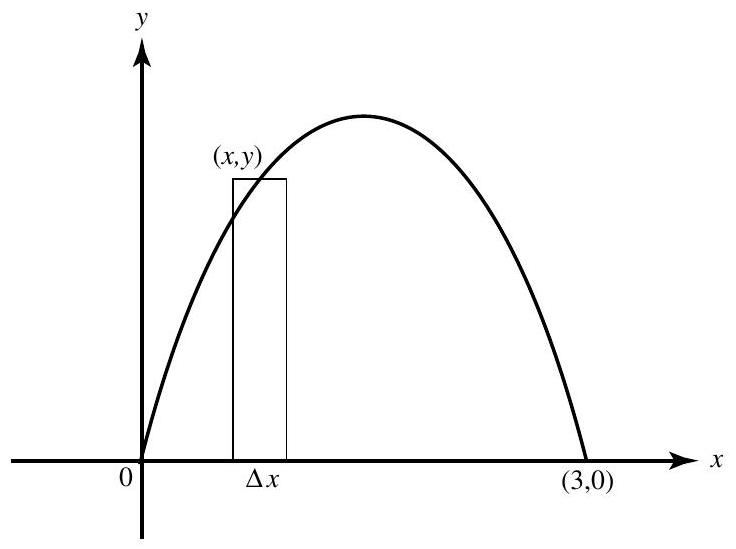
\includegraphics[width=0.50\linewidth]{calculus/images/4dd14383-56bc-4a03-ad67-ca78eb85270b-25_549_736_1878_487.jpg}
\end{center}
About the $x$-axis.\\
Disk.
\[
\begin{aligned}
\Delta V & =\pi y^{2} \Delta x \\
& =\pi\left(3 x-x^{2}\right)^{2} \Delta x
\end{aligned}
\]
$\pi \int_{0}^{3}\left(3 x-x^{2}\right)^{2} d x$
\end{solution}

\newpage



\question
$y=3 x-x^{2}$ and $y=x$; about the $x$-axis.
\begin{choices}
  \choice $\pi \int_{0}^{3 / 2}\left[\left(3 x-x^{2}\right)^{2}-x^{2}\right] d x$
  \choice $\pi \int_{0}^{2}\left(9 x^{2}-6 x^{3}\right) d x$
  \CorrectChoice $\pi \int_{0}^{2}\left[\left(3 x-x^{2}\right)^{2}-x^{2}\right] d x$
  \choice $\pi \int_{0}^{3}\left[\left(3 x-x^{2}\right)^{2}-x^{4}\right] d x$
  \choice $\pi \int_{0}^{3}\left(2 x-x^{2}\right)^{2} d x$
\end{choices}
\begin{solution}
(C)
\begin{center}
  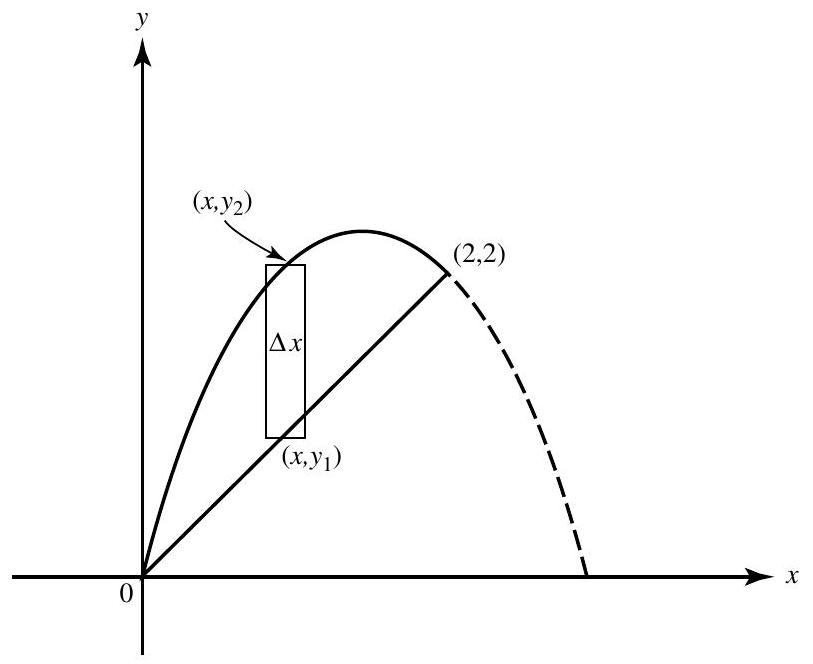
\includegraphics[width=0.50\linewidth]{calculus/images/4dd14383-56bc-4a03-ad67-ca78eb85270b-26_664_813_299_825.jpg}
\end{center}
About the $x$-axis.\\
Washer.
\[
\begin{aligned}
& \Delta V=\pi y_{2}^{2} \Delta x-\pi y_{1}^{2} \Delta x \\
& \quad=\pi\left[\left(3 x-x^{2}\right)^{2}-x^{2}\right] \Delta x \\
& \pi \int_{0}^{2}\left[(3 x-x)^{2}-x^{2}\right] d x
\end{aligned}
\]
\end{solution}

\newpage



\question
$y=\ln x, y=0, x=e$; about the line $x=e$.
\begin{choices}
  \choice $\pi \int_{1}^{e}(e-x) \ln x d x$
  \CorrectChoice $\pi \int_{0}^{1}\left(e-e^{y}\right)^{2} d y$
  \choice $2 \pi \int_{1}^{e}(e-\ln x) d x$
  \choice $\pi \int_{0}^{e}\left(e^{2}-2 e^{y+1}+e^{2 y}\right) d y$
  \choice none of these
\end{choices}
\begin{solution}
\begin{center}
  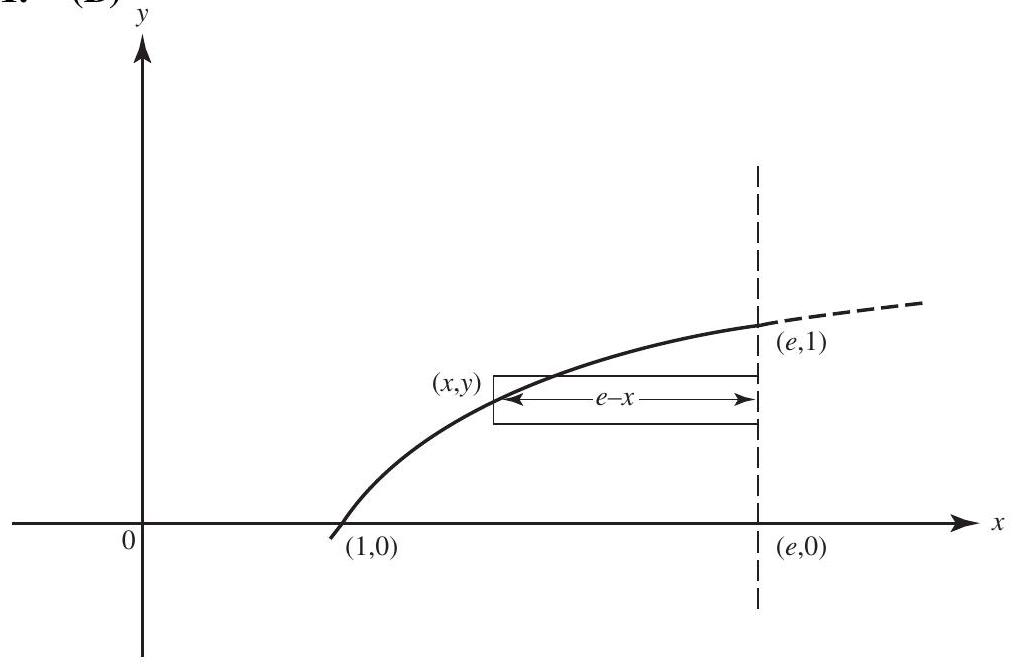
\includegraphics[width=0.50\linewidth]{calculus/images/4dd14383-56bc-4a03-ad67-ca78eb85270b-26_664_1017_1041_693.jpg}
\end{center}
About $x=e$.\\
Disk.
\[
\begin{aligned}
& \Delta V=\pi(e-x)^{2} \Delta y \\
&=\pi\left(e-e^{y}\right)^{2} \Delta y \\
& \pi \int_{0}^{1}\left(e-e^{y}\right)^{2} d y
\end{aligned}
\]
\end{solution}

\newpage


\question
The curve with parametric equations $x=\tan \theta, y=\cos ^{2} \theta$, and the lines $x=0$, $x=1$, and $y=0$; about the $x$-axis.
\begin{choices}
  \choice $\pi \int_{0}^{\pi / 4} \cos ^{4} \theta d \theta$
  \choice $\pi \int_{0}^{\pi / 4} \cos ^{2} \theta \sin \theta d \theta$
  \CorrectChoice $\pi \int_{0}^{\pi / 4} \cos ^{2} \theta d \theta$
  \choice $\pi \int_{0}^{1} \cos ^{2} \theta d \theta$
  \choice $\pi \int_{0}^{1} \cos ^{4} \theta d \theta$
\end{choices}
\begin{solution}
About the $x$-axis.
Disk.
$\Delta V=\pi y^{2} \Delta x$.
$\pi \int_{0}^{1} y^{2} d x=\pi \int_{0}^{\pi / 4} \cos ^{2} \theta d \theta$
\end{solution}

\question
A sphere of radius $r$ is divided into two parts by a plane at distance $h(0<h<r)$ from the center. The volume of the smaller part equals
\begin{choices}
  \CorrectChoice $\dfrac{\pi}{3}\left(2 r^{3}+h^{3}-3 r^{2} h\right)$
  \choice $\dfrac{\pi h}{3}\left(3 r^{2}-h^{2}\right)$
  \choice $\dfrac{4}{3} \pi r^{3}+\dfrac{h^{3}}{3}-r^{2} h$
  \choice $\dfrac{\pi}{3}\left(2 r^{3}+3 r^{2} h-h^{3}\right)$
  \choice none of these
\end{choices}
\begin{solution}
  \begin{center}
    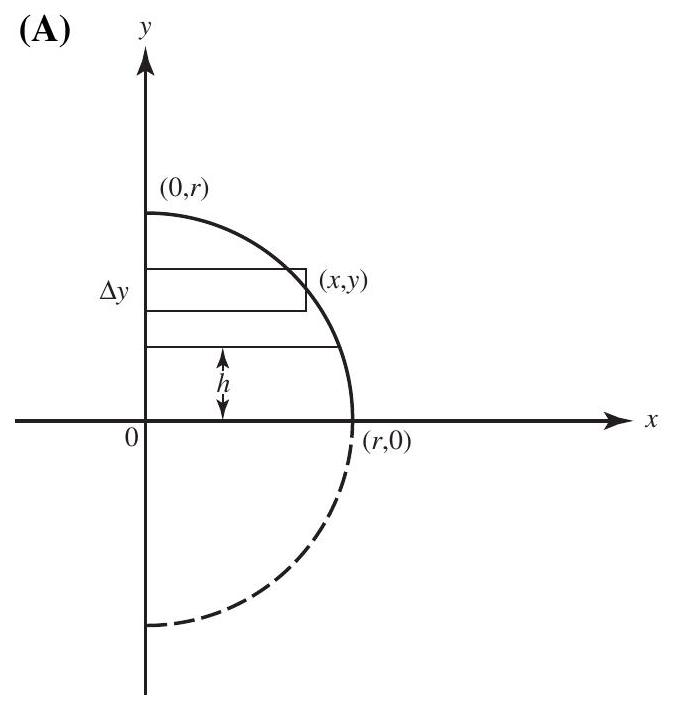
\includegraphics[width=0.40\linewidth]{calculus/images/4dd14383-56bc-4a03-ad67-ca78eb85270b-27_709_675_289_379.jpg}
  \end{center}  
  About the $y$-axis.\\
  Disk.  
  \[
  \begin{aligned}
  \Delta V & =\pi x^{2} \Delta y \\
  & =\pi\left(r^{2}-y^{2}\right) \Delta y
  \end{aligned}
  \]
  $\pi \int_{h}^{r}\left(r^{2}-y^{2}\right) d y=\dfrac{\pi}{3}\left(2 r^{3}+h^{3}-3 r^{2} h\right)$
\end{solution}


\newpage


\question\label{calc07:volume2-last}
If the curves of $f(x)$ and $g(x)$ intersect for $x=a$ and $x=b$ and if $f(x)>g(x)>0$ for all $x$ on $(a, b)$, then the volume obtained when the region bounded by the curves is rotated about the $x$-axis is equal to
\begin{choices}
  \choice $\pi \int_{a}^{b} f^{2}(x) d x-\int_{a}^{b} g^{2}(x) d x$
  \choice $\pi \int_{a}^{b}[f(x)-g(x)]^{2} d x$
  \choice $2 \pi \int_{a}^{b} x[f(x)-g(x)] d x$
  \CorrectChoice $\pi \int_{a}^{b}\left[f^{2}(x)-g^{2}(x)\right] d x$
  \choice none of these


\end{choices}
\begin{solution}
(D)
\begin{center}
  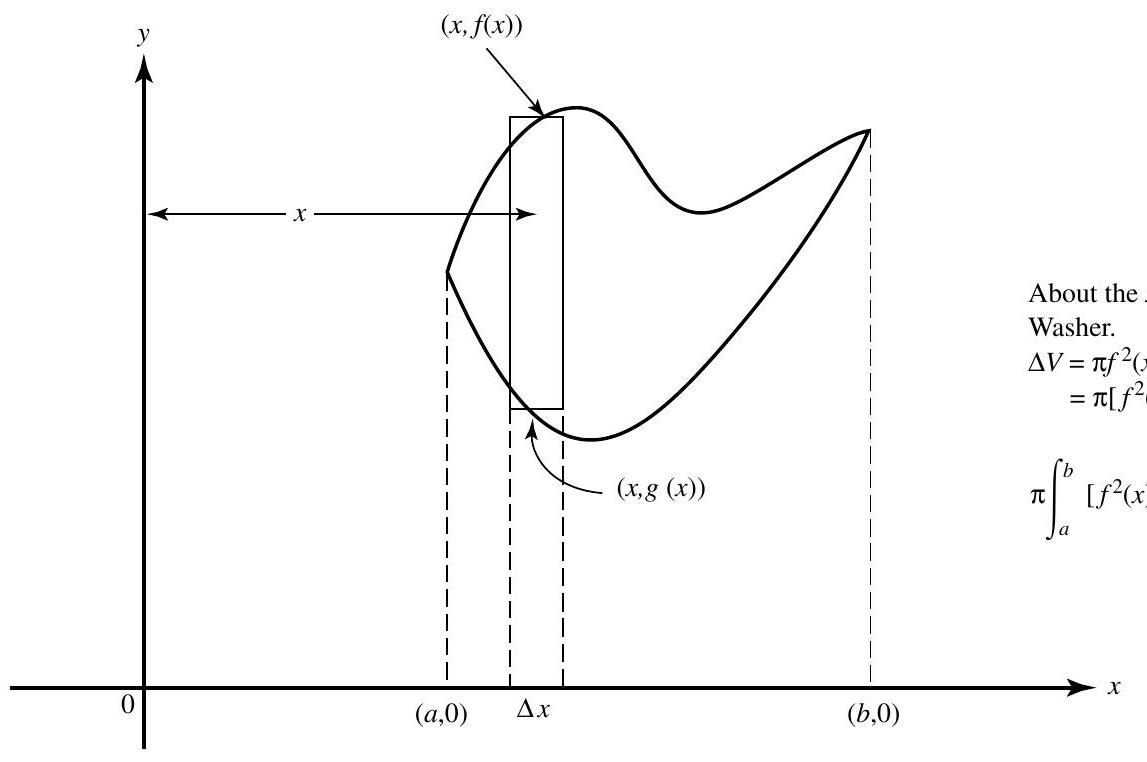
\includegraphics[width=0.50\linewidth]{calculus/images/4dd14383-56bc-4a03-ad67-ca78eb85270b-27_762_1147_1080_315.jpg}
\end{center}

\end{solution}

\question
The length of one arch of the cycloid $\begin{aligned} & x=t-\sin t \\ & y=1-\cos t\end{aligned}$ equals
\begin{choices}
  \choice $\int_{0}^{\pi} \sqrt{1-\cos t} d t$
  \choice $\int_{0}^{2 \pi} \sqrt{\dfrac{1-\cos t}{2}} d t$
  \choice $\int_{0}^{\pi} \sqrt{2-2 \cos t} d t$
  \CorrectChoice $\int_{0}^{2 \pi} \sqrt{2-2 \cos t} d t$
  \choice $2 \int_{0}^{\pi} \sqrt{\dfrac{1-\cos t}{2}} d t$
\end{choices}
\begin{solution}
From (3) on page 305, we obtain the length:
\[
\int_{0}^{2 \pi} \sqrt{(1-\cos t)^{2}+(\sin t)^{2}} d t=\int_{0}^{2 \pi} \sqrt{2-2 \cos t} d t
\]
\end{solution}





\newpage





\question
The length of the arc of the parabola $4 x=y^{2}$ cut off by the line $x=2$ is given by the integral
\begin{choices}
  \choice $\int_{-1}^{1} \sqrt{x^{2}+1} d x$
  \choice $\dfrac{1}{2} \int_{0}^{2} \sqrt{4+y^{2}} d y$
  \choice $\int_{-1}^{1} \sqrt{1+x} d x$
  \CorrectChoice $\int_{0}^{2 \sqrt{2}} \sqrt{4+y^{2}} d y$
  \choice none of these
\end{choices}
\begin{solution}
Note that the curve is symmetric to the $x$-axis. Use (2) on page 305.
\end{solution}

\question
The length of $x=e^{t} \cos t, y=e^{t} \sin t$ from $t=2$ to $t=3$ is equal to
\begin{choices}
  \choice $\sqrt{2} e^{2} \sqrt{e^{2}-1}$
  \CorrectChoice $\sqrt{2}\left(e^{3}-e^{2}\right)$
  \choice $2\left(e^{3}-e^{2}\right)$
  \choice $e^{3}(\cos 3+\sin 3)-e^{2}(\cos 2+\sin 2)$
  \choice none of these



\end{choices}
\begin{solution}
Use (3) on page 305 to get the integral:


\[
\int_{2}^{3} \sqrt{\left(-e^{t} \sin t+e^{t} \cos t\right)^{2}+\left(e^{t} \cos t+e^{t} \sin t\right)^{2}} d t=\left.\sqrt{2} e^{t}\right|_{2} ^{3}
\]


\end{solution}

\question
Which one of the following is an improper integral?
\begin{choices}
  \choice $\int_{0}^{2} \dfrac{d x}{\sqrt{x+1}}$
  \choice $\int_{-1}^{1} \dfrac{d x}{1+x^{2}}$
  \CorrectChoice $\int_{0}^{2} \dfrac{x d x}{1-x^{2}}$
  \choice $\int_{0}^{\pi / 3} \dfrac{\sin x d x}{\cos ^{2} x}$
  \choice none of these
\end{choices}
\begin{solution}
The integrand is discontinuous at $x=1$, which is on the interval of integration.
\end{solution}



\newpage



\question
Which one of the following improper integrals diverges?
\begin{choices}
  \choice $\int_{1}^{\infty} \dfrac{d x}{x^{2}}$
  \choice $\int_{0}^{\infty} \dfrac{d x}{e^{x}}$
  \choice $\int_{-1}^{1} \dfrac{d x}{\sqrt[3]{x}}$
  \CorrectChoice $\int_{-1}^{1} \dfrac{d x}{x^{2}}$
  \choice none of these
\end{choices}
\begin{solution}
The integral in (D) is the sum of two integrals from -1 to 0 and from 0 to 1. Both diverge (see Example 29, pages 312 and 313). Note that (A), (B), and (C) all converge.
\end{solution}

\question
Which one of the following improper integrals diverges?
\begin{choices}
  \choice $\int_{0}^{\infty} \dfrac{d x}{1+x^{2}}$
  \choice $\int_{0}^{1} \dfrac{d x}{x^{1 / 3}}$
  \choice $\int_{0}^{\infty} \dfrac{d x}{x^{3}+1}$
  \choice $\int_{0}^{\infty} \dfrac{d x}{e^{x}+2}$
  \CorrectChoice $\int_{1}^{\infty} \dfrac{d x}{x^{1 / 3}}$

\end{choices}
\begin{solution}
Choices (A), (C), and (D) can be shown convergent by the Comparison Test; the convergence of (B) is shown in Example 24, page 311.

\end{solution}
